% template by Natalia Chernov for the University of Oldenburg

\documentclass[xcolor=table,9pt,aspectratio=169]{beamer}

\usepackage[utf8]{inputenc}

\usepackage{amsmath}
\usepackage{anyfontsize}
\usepackage[english,ngerman]{babel}
\usepackage[autostyle]{csquotes}
\usepackage{datetime}
\usepackage{helvet}
   \renewcommand{\familydefault}{\sfdefault}
\usepackage{hyperref}
   \urlstyle{same}
\usepackage{lipsum}
\usepackage{listings}
\usepackage{lmodern}
\usepackage{multicol}
\usepackage{multirow}
\usepackage{smartdiagram}
\usepackage{tikz}
\usepackage{xcolor}

\definecolor{uolblue}{RGB}{0,62,107}

\definecolor{blue1}{RGB}{0,78,159}
\definecolor{blue2}{RGB}{0,171,217}
\definecolor{blue3}{RGB}{91,197,242}
\definecolor{blue4}{RGB}{161,217,248}

\definecolor{green1}{RGB}{0,120,120}
\definecolor{green2}{RGB}{0,168,121}
\definecolor{green3}{RGB}{148,193,28}
\definecolor{green4}{RGB}{199,211,0}

\definecolor{orange1}{RGB}{213,59,10}
\definecolor{orange2}{RGB}{238,113,0}
\definecolor{orange3}{RGB}{243,145,0}
\definecolor{orange4}{RGB}{253,195,0}

\definecolor{gr}{RGB}{191,191,191}
\definecolor{grcode}{RGB}{190,190,190}

\lstdefinestyle{mystyle}{
   backgroundcolor=\color{grcode},
   commentstyle=\color{blue1},
   numberstyle=\tiny\color{blue1},
   basicstyle=\ttfamily\footnotesize,
   breakatwhitespace=false,
   breaklines=true,
   captionpos=b,
   keepspaces=true,
   numbers=left,
   numbersep=5pt,
   showspaces=false,
   showstringspaces=false,
   showtabs=false,
   tabsize=2
}

\setbeameroption{hide notes}
% \setbeameroption{show only notes}
% \setbeameroption{show notes on second screen=right}

\setbeamertemplate{frametitle}{\color{uolblue}\fontsize{12}{20}\selectfont{\insertframetitle}}

\pgfdeclareimage[width=0.145\paperwidth]{logo}{figures/logo_uol_negative}
\pgfdeclareimage[width=0.072\paperwidth]{logo_small}{figures/logo_uol_negative}

\defbeamertemplate*{background canvas}{default_page}
{%
\begin{tikzpicture}
   \useasboundingbox (0,0) rectangle (\the\paperwidth,\the\paperheight);
   \filldraw[fill=uolblue,fill opacity=1,draw=none] (0,0) rectangle (0.119\paperwidth,\the\paperheight);
   \filldraw[fill=blue2,fill opacity=1,draw=none] (0.119\paperwidth,0) -- (0.119\paperwidth,0.565\paperheight) arc (117.2:180:0.6\paperwidth) -- cycle;
   \pgftext[at=\pgfpoint{10}{\the\paperheight-11.5},left,top]{\pgfsetfillopacity{1}\pgfuseimage{logo_small}};
\end{tikzpicture}
}
\defbeamertemplate*{background canvas}{titlepage_image}
{
\begin{tikzpicture}
   \useasboundingbox (0,0) rectangle (\the\paperwidth,\the\paperheight);
   \filldraw[fill=uolblue,fill opacity=1,draw=none] (0,0) rectangle (\the\paperwidth,\the\paperheight);
   \filldraw[fill=blue2,fill opacity=1,draw=none] (\the\paperwidth,0) -- (\the\paperwidth,0.66\paperheight) arc (90:180:0.6\paperwidth) -- cycle;
   \pgftext[at=\pgfpoint{14}{\the\paperheight-17.5},left,top]{\pgfsetfillopacity{1}\pgfuseimage{logo}};
\end{tikzpicture}
}
\BeforeBeginEnvironment{frame}{%
   \setbeamertemplate{background canvas}[default_page]%
}
\makeatletter
\define@key{beamerframe}{titlepage_image}[true]{%
   \setbeamercovered{invisible}%
   \setbeamertemplate{background canvas}[titlepage_image]%
}
\makeatother%

\setbeamertemplate{footline}
{
   \leavevmode
   \hbox{
   \hspace*{.025\paperwidth}\begin{beamercolorbox}[wd=.094\paperwidth,ht=2.25ex,dp=1ex,left]{}
   ~

   \vspace*{.042\paperheight}
      \fontsize{4.4}{5.9}\selectfont\color{white}\textbf{Folie \insertframenumber}\newline\insertdate
   \vspace*{.026\paperheight}
   \end{beamercolorbox}
   \hspace*{.05\paperwidth}\begin{beamercolorbox}
   [wd=.79\paperwidth,ht=2.25ex,dp=1ex,left]{}
   ~

   \vspace*{.042\paperheight}
      \fontsize{4.4}{5.9}\selectfont\color{black}\textbf{Forschungsorientierte Einführung in die Experimentelle Philosophie}\newline\color{gray}\insertauthor~--~Fakultät IV, Institut für Philosophie
   \vspace*{.026\paperheight}
   \end{beamercolorbox}
   }
   \vskip0pt
}

\setbeamerfont{title}{size={\fontsize{22}{25}}}
\setbeamerfont{subtitle}{size={\fontsize{12}{14}}}
\setbeamerfont{author}{size={\fontsize{9}{11}}}
\setbeamerfont{date}{size={\fontsize{9}{11}}}
\setbeamercolor{title}{fg=white}
\setbeamercolor{subtitle}{fg=white}
\setbeamercolor{author}{fg=white}
\setbeamercolor{date}{fg=white}
\setbeamercolor{color_Logo-Platzhalter}{fg=white,bg=gray!40}

\defbeamertemplate*{title page}{customized}[1][]
{  \vspace*{20mm}
   \hspace*{-22.5mm}
   \begin{minipage}{\textwidth}
   \usebeamerfont{title}\usebeamercolor[fg]{title}\inserttitle\par
   \bigskip
   \usebeamerfont{subtitle}\usebeamercolor[fg]{subtitle}\insertsubtitle\par
   \bigskip
   \usebeamerfont{author}\usebeamercolor[fg]{author}\insertauthor\par
   \bigskip
   \usebeamerfont{date}\usebeamercolor[fg]{date}\insertdate\par
   \end{minipage}
}
\setbeamertemplate{navigation symbols}{}
\setbeamersize{text margin left=0.17\paperwidth,text margin right=0.04\paperwidth}

\title{Forschungsorientierte Einführung in \\die Experimentelle Philosophie}
\subtitle{}
\author{Alexander Max Bauer und Stephan Kornmesser}
\date{SoSe 2024}
% \date{\renewcommand{\dateseparator}{.}\ddmmyyyydate\today}
\usepackage{enumitem}
\def\labelitemi{--}
\def\labelitemii{--}
\def\labelitemiii{--}

\begin{document}
{
\setbeamertemplate{footline}{}
\begin{frame}[titlepage_image]
   \maketitle
\end{frame}
}

%%%%%%%%%%%%%%%%%%%%%%%%
% FOLIE 2 – GLIEDERUNG %
%%%%%%%%%%%%%%%%%%%%%%%%
\begin{frame}{\vspace*{10mm}Gliederung}
\begin{itemize}
   \item[1] Einführung und Organisatorisches
   \begin{itemize}
      \item Modulzuordnung und Prüfungsformen
      \item Seminarstruktur
      \item Klassisches Beispiel aus der Experimentellen Philosophie
   \end{itemize}
   \item[2] Vorbereitung der Replikationsstudie
   \begin{itemize}
      \item Originalstudie
      \item Problemstruktur
      \item Studienaufbau
      \item Vignette (Original)
      \item Vignette (Übersetzung)
      \item Umfragematerial
   \end{itemize}
\end{itemize}
\end{frame}


%%%%%%%%%%%
% FOLIE 3 %
%%%%%%%%%%%
\begin{frame}{\vspace*{10mm}Gliederung}
\begin{itemize}
   \item[3] Analyse der Replikationsstudie
   \begin{itemize}
      \item Datengrundlage
      \item Beobachtete Häufigkeiten
      \item Hypothese
      \item Erwartete Häufigkeiten bei Unabhängigkeit
      \item Berechnung der Residuen
      \item Berechnung der $\chi^{2}$-Statistik
      \item $\chi^2$-Verteilung
      \item Signifikanzniveau
      \item Online-$\chi^2$-Rechner
   \end{itemize}
   \item[4] Ergebnisse der Replikationsstudie
   \begin{itemize}
      \item Offene Wissenschaft und offene Daten
      \item Auswertung mit R
      \item Ergebnisse der Gruppen
   \end{itemize}
\end{itemize}
\end{frame}


%%%%%%%%%%%
% FOLIE 4 %
%%%%%%%%%%%
\begin{frame}{\vspace*{10mm}Gliederung}
\begin{itemize}
   \item[5] Vorbereitung der eigenen Themen
   \begin{itemize}
      \item Gruppenzuordnung
      \item Recherche
   \end{itemize}
   \item[6] Analyse der eigenen Themen
   \begin{itemize}
      \item Struktur
   \end{itemize}
\end{itemize}
\end{frame}


%%%%%%%%%%%%%%%%%%%%%%%%
% FOLIE 5 – EINFÜHRUNG %
%%%%%%%%%%%%%%%%%%%%%%%%
\begin{frame}
\begin{overlayarea}{\textwidth}{0.81\paperheight}{
   \vspace*{11mm}
   \usebeamerfont{title}\textcolor{uolblue}
   {1\hspace*{1em}Einführung und Organisatorisches}
}
\end{overlayarea}
\end{frame}


%%%%%%%%%%%
% FOLIE 6 %
%%%%%%%%%%%
\begin{frame}{\vspace*{10mm}1\hspace*{1em}Einführung und Organisatorisches}
\textbf{Modulzuordnung und Prüfungsformen}\\
\begin{itemize}
   \item \textbf{phi331:} Theoretische Philosophie und ihre Konsequenzen für die\\Grundlagen der Wissenschaften
   \begin{itemize}
      \item Hausarbeit \textcolor{gray}{(16\,--\,18 Seiten)}
      \item Referat \textcolor{gray}{(30\,--\,35 Minuten)} mit schriftlicher Ausarbeitung \textcolor{gray}{(10\,--\,12 Seiten)}
      \item Mündliche Prüfung \textcolor{gray}{(25\,--\,30 Minuten)}
   \end{itemize}
   \item \textbf{phi530:} Theoretische Philosophie und Grundlagen der Wissenschaften
   \item \textbf{phi540:} Akzentuierung
   \begin{itemize}
      \item Hausarbeit \textcolor{gray}{(18\,--\,20 Seiten)}
      \item Referat \textcolor{gray}{(40\,--\,45 Minuten)} mit schriftlicher Ausarbeitung \textcolor{gray}{(12\,--\,14 Seiten)}
      \item Mündliche Prüfung \textcolor{gray}{(30\,--\,35 Minuten)}
   \end{itemize}
\end{itemize}
\end{frame}


%%%%%%%%%%%
% FOLIE 7 %
%%%%%%%%%%%
\begin{frame}{\vspace*{10mm}1\hspace*{1em}Einführung und Organisatorisches}
\textbf{Seminarstruktur}\\
\begin{flushleft}
   \smartdiagramset{uniform sequence color=true,
   sequence item uniform color=blue2,
   sequence item border color=white,
   sequence item font size=\footnotesize,
   sequence item text color=white,
   sequence item height=1.5cm,
   sequence item width=1.8cm
   }
   \smartdiagram[sequence diagram]{Replikations\-studie zum Einstieg,Formulierung eigener Forschungsfrage,Umsetzung und Durchführung eigener Studie,Analyse und Interpretation eigener Studie}
\end{flushleft}
\end{frame}


%%%%%%%%%%%
% FOLIE 8 %
%%%%%%%%%%%
\begin{frame}{\vspace*{10mm}1\hspace*{1em}Einführung und Organisatorisches}
\textbf{Klassisches Beispiel aus der Experimentellen Philosophie}\\
\begin{multicols}{2}
   \begin{center}
      \frame{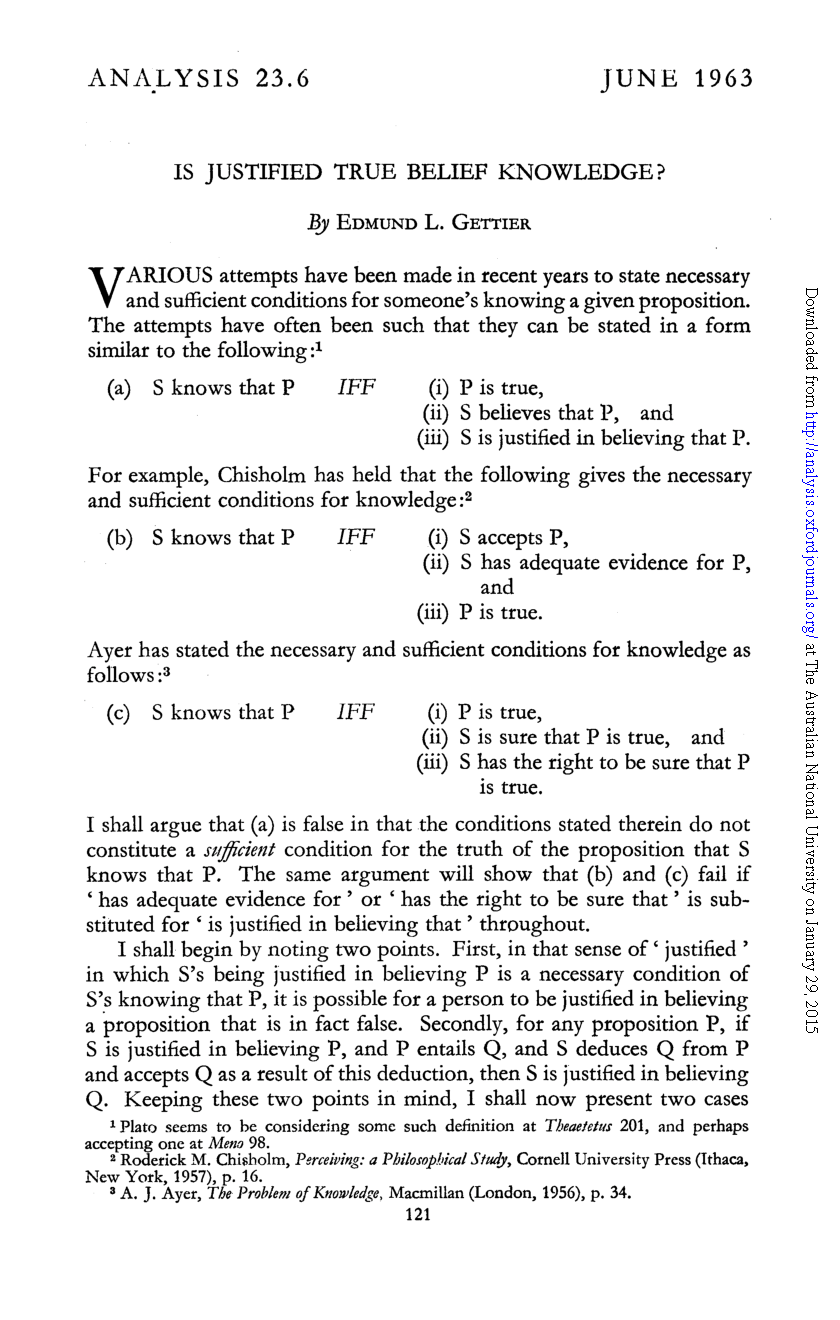
\includegraphics[width=0.5\linewidth]{figures/paper_gettier_1963.pdf}}\\
      \textcolor{gray}{Gettier (1963)}\\
      \frame{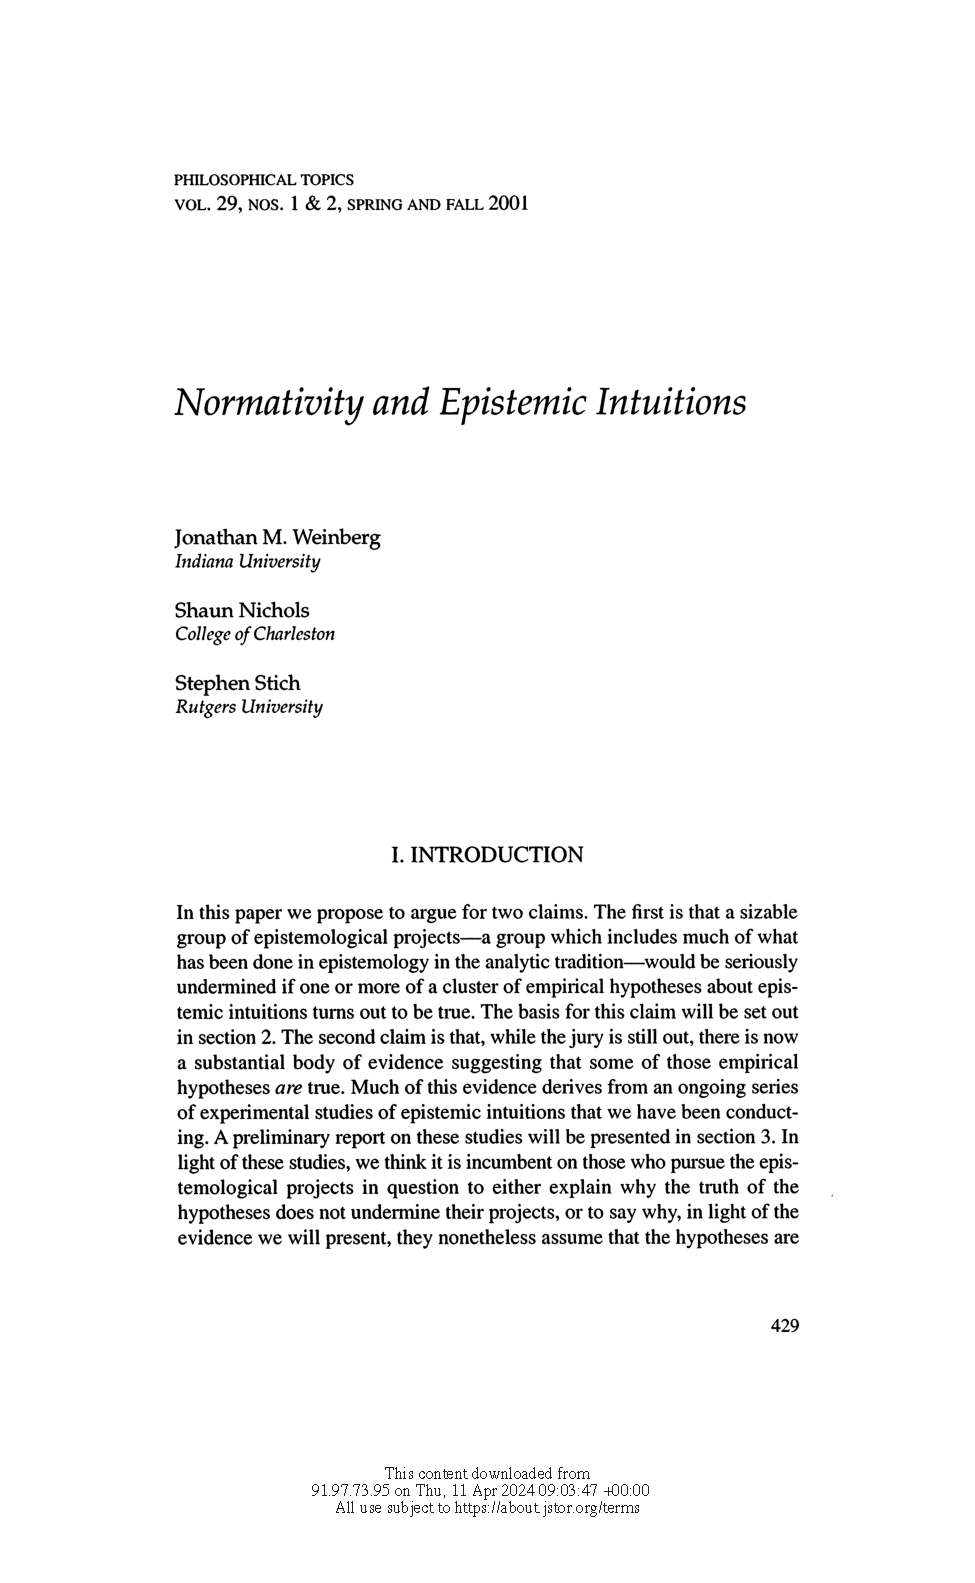
\includegraphics[width=0.5\linewidth]{figures/paper_weinberg_2001.pdf}}\\
      \textcolor{gray}{Weinberg, Nichols und Stich (2001)}
   \end{center}
\end{multicols}
\end{frame}


%%%%%%%%%%%%%%%%%%%%%%%%%%%%%%%%%%%%%%
% FOLIE 9 – VORBEREITUNG REPLIKATION %
%%%%%%%%%%%%%%%%%%%%%%%%%%%%%%%%%%%%%%
\begin{frame}
\begin{overlayarea}{\textwidth}{0.81\paperheight}{
   \vspace*{11mm}
   \usebeamerfont{title}\textcolor{uolblue}
   {2\hspace*{1em}Vorbereitung der Replikationsstudie}
}
\end{overlayarea}
\end{frame}


%%%%%%%%%%%%
% FOLIE 10 %
%%%%%%%%%%%%
\begin{frame}{\vspace*{10mm}2\hspace*{1em}Vorbereitung der Replikationsstudie}
\textbf{Originalstudie}\\
\begin{center}
   \frame{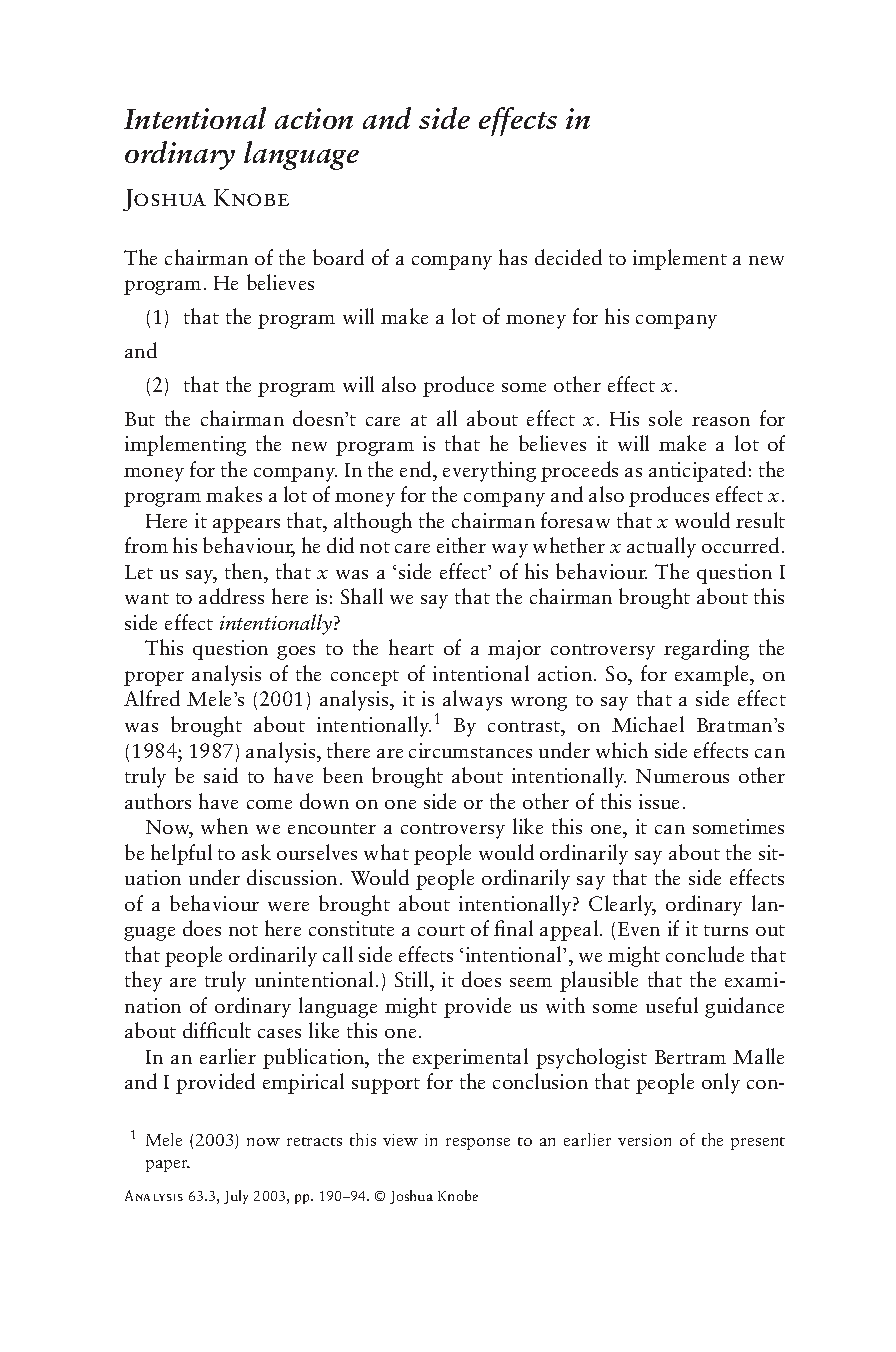
\includegraphics[width=0.25\linewidth]{figures/paper_knobe_2003.pdf}}\\
   \textcolor{gray}{Knobe (2003)}
\end{center}
\end{frame}


%%%%%%%%%%%%
% FOLIE 11 %
%%%%%%%%%%%%
\begin{frame}{\vspace*{10mm}2\hspace*{1em}Vorbereitung der Replikationsstudie}
\textbf{Problemstruktur}\\
\begin{center}
   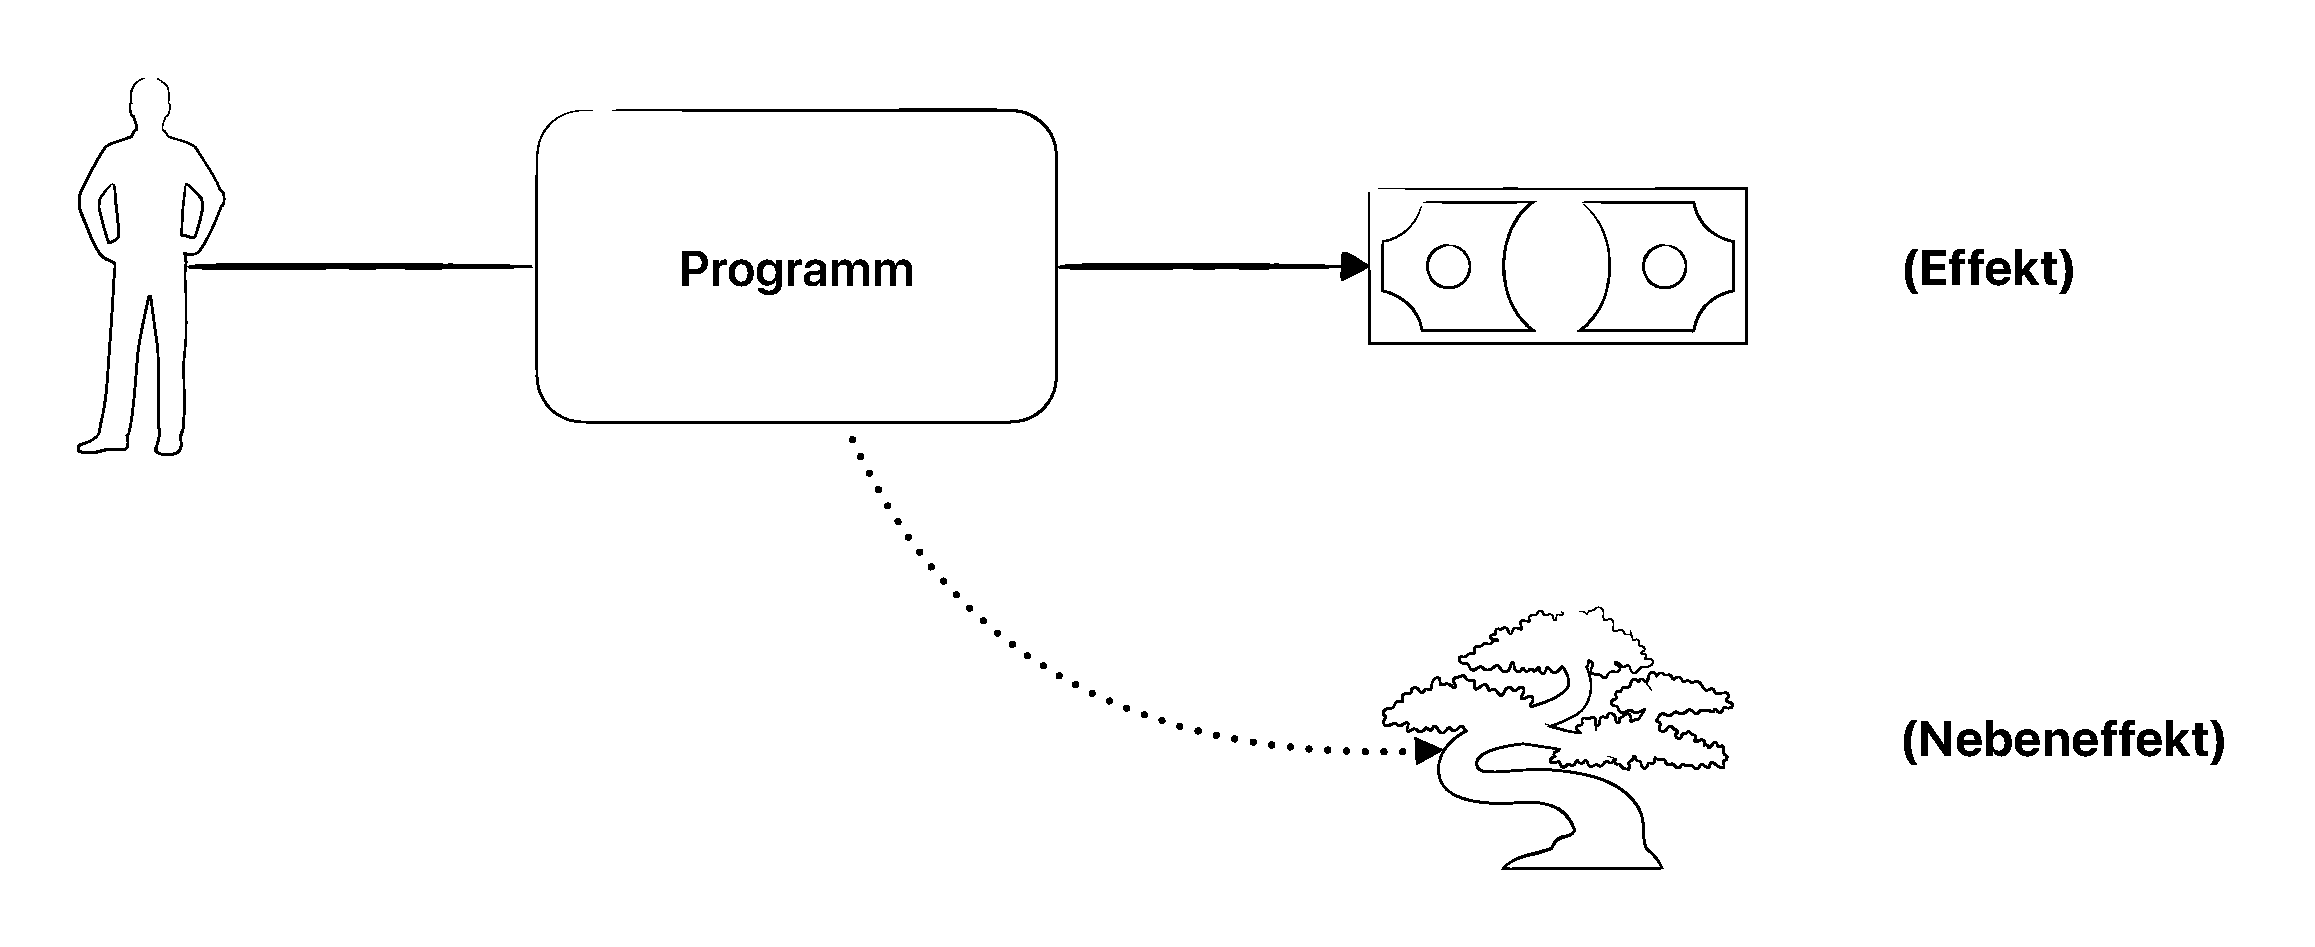
\includegraphics[width=0.75\linewidth]{figures/replication_knobe_structure.pdf}\\
\end{center}
\enquote{Shall we say that the chairman brought about this side effect \textit{intentionally}?}\\
\textcolor{gray}{(Knobe 2003, S.~190)}
\bigskip
\end{frame}


%%%%%%%%%%%%
% FOLIE 12 %
%%%%%%%%%%%%
\begin{frame}{\vspace*{10mm}2\hspace*{1em}Vorbereitung der Replikationsstudie}
\textbf{Studienaufbau}\\
\begin{itemize}
   \item Zwei Varianten einer Vignette \textcolor{gray}{(Entscheidung schadet oder hilft der Umwelt)}
   \item Teilnehmer*innen sehen immer nur eine Variante der Vignette \textcolor{gray}{(\enquote{between subjects})}
   \item Im Anschluss zwei Fragen
   \begin{itemize}
      \item Wie tadelns- oder lobenswert ist die Person für ihre Entscheidung? \textcolor{gray}{(Skala von~0 bis~6)}
      \item Hat die Person den Nebeneffekt absichtlich herbeigeführt? \textcolor{gray}{(ja oder nein)}
   \end{itemize}
\end{itemize}
\end{frame}


%%%%%%%%%%%%
% FOLIE 13 %
%%%%%%%%%%%%
\begin{frame}{\vspace*{10mm}2\hspace*{1em}Vorbereitung der Replikationsstudie}
\textbf{Vignette (Original)}\\
\smallskip
\enquote{The vice-president of a company went to the chairman of the board and said, \enquote{We are thinking of starting a new program. It will help us increase profits, but \textcolor{blue2}{[and]} it will also harm \textcolor{blue2}{[help]} the environment.}\\\vspace{0.25em}
The chairman of the board answered, \enquote{I don't care at all about harming \textcolor{blue2}{[helping]} the environment. I just want to make as much profit as I can. Let's start the new program.}\\\vspace{0.25em}
They started the new program. Sure enough, the environment was harmed \textcolor{blue2}{[helped]}.}\\
\textcolor{gray}{(Knobe 2003, S.~190)}

\bigskip
\textbf{Fragen (Original)}\\
\begin{itemize}
   \item \enquote{These subjects were then asked to determine how much blame \textcolor{blue2}{[praise]} the chairman deserved for what he did (on a scale from 0 to 6)} \textcolor{gray}{(ebd., S.~191\,f.)}
   \item \enquote{These subjects were then asked [$\ldots$] to say whether they thought the chairman \textit{intentionally} harmed the environment} \textcolor{gray}{(ebd. S.~191)}
\end{itemize}
\end{frame}


%%%%%%%%%%%%
% FOLIE 14 %
%%%%%%%%%%%%
\begin{frame}{\vspace*{10mm}2\hspace*{1em}Vorbereitung der Replikationsstudie}
\textbf{Vignette (Übersetzung)}\\
\smallskip
\enquote{Der Vizepräsident eines Unternehmens ging zum Vorstandsvorsitzenden und sagte: \enquote{Wir überlegen uns, ein neues Programm ins Leben zu rufen. Es wird uns dabei helfen, die Gewinne zu steigern, aber \textcolor{blue2}{[und]} es wird auch die Umwelt schädigen \textcolor{blue2}{[schützen]}.}\\\vspace{0.25em}
Der Vorstandsvorsitzende antwortete: \enquote{Es ist mir völlig gleichgültig, ob die Umwelt geschädigt \textcolor{blue2}{[geschützt]} wird. Ich will nur so viel Gewinn machen wie möglich. Beginnen wir also mit dem neuen Programm.}\\\vspace{0.25em}
Sie begannen mit dem neuen Programm. Und tatsächlich wurde die Umwelt geschädigt \textcolor{blue2}{[geschützt]}.} \textcolor{gray}{(Knobe 2014, S.~98)}

\bigskip
\textbf{Fragen (Übersetzung)}\\
\begin{itemize}
   \item \enquote{Die Versuchspersonen wurden dann gebeten, zu entscheiden, wie viel Tadel \textcolor{blue2}{[Lob]} der Vorstandsvorsitzende für sein Handeln verdiente (auf einer Skala von 0 bis 6)} \textcolor{gray}{(ebd.)}
   \item \enquote{Die Versuchspersonen wurden dann gebeten, zu [$\ldots$] sagen, ob sie dachten, dass der Vorsitzende die Umwelt \textit{absichtlich} schädigte} \textcolor{gray}{(ebd.)}
\end{itemize}
\end{frame}


%%%%%%%%%%%%
% FOLIE 15 %
%%%%%%%%%%%%
\begin{frame}{\vspace*{10mm}2\hspace*{1em}Vorbereitung der Replikationsstudie}
\textbf{Umfragematerial}\\
\begin{center}
   \frame{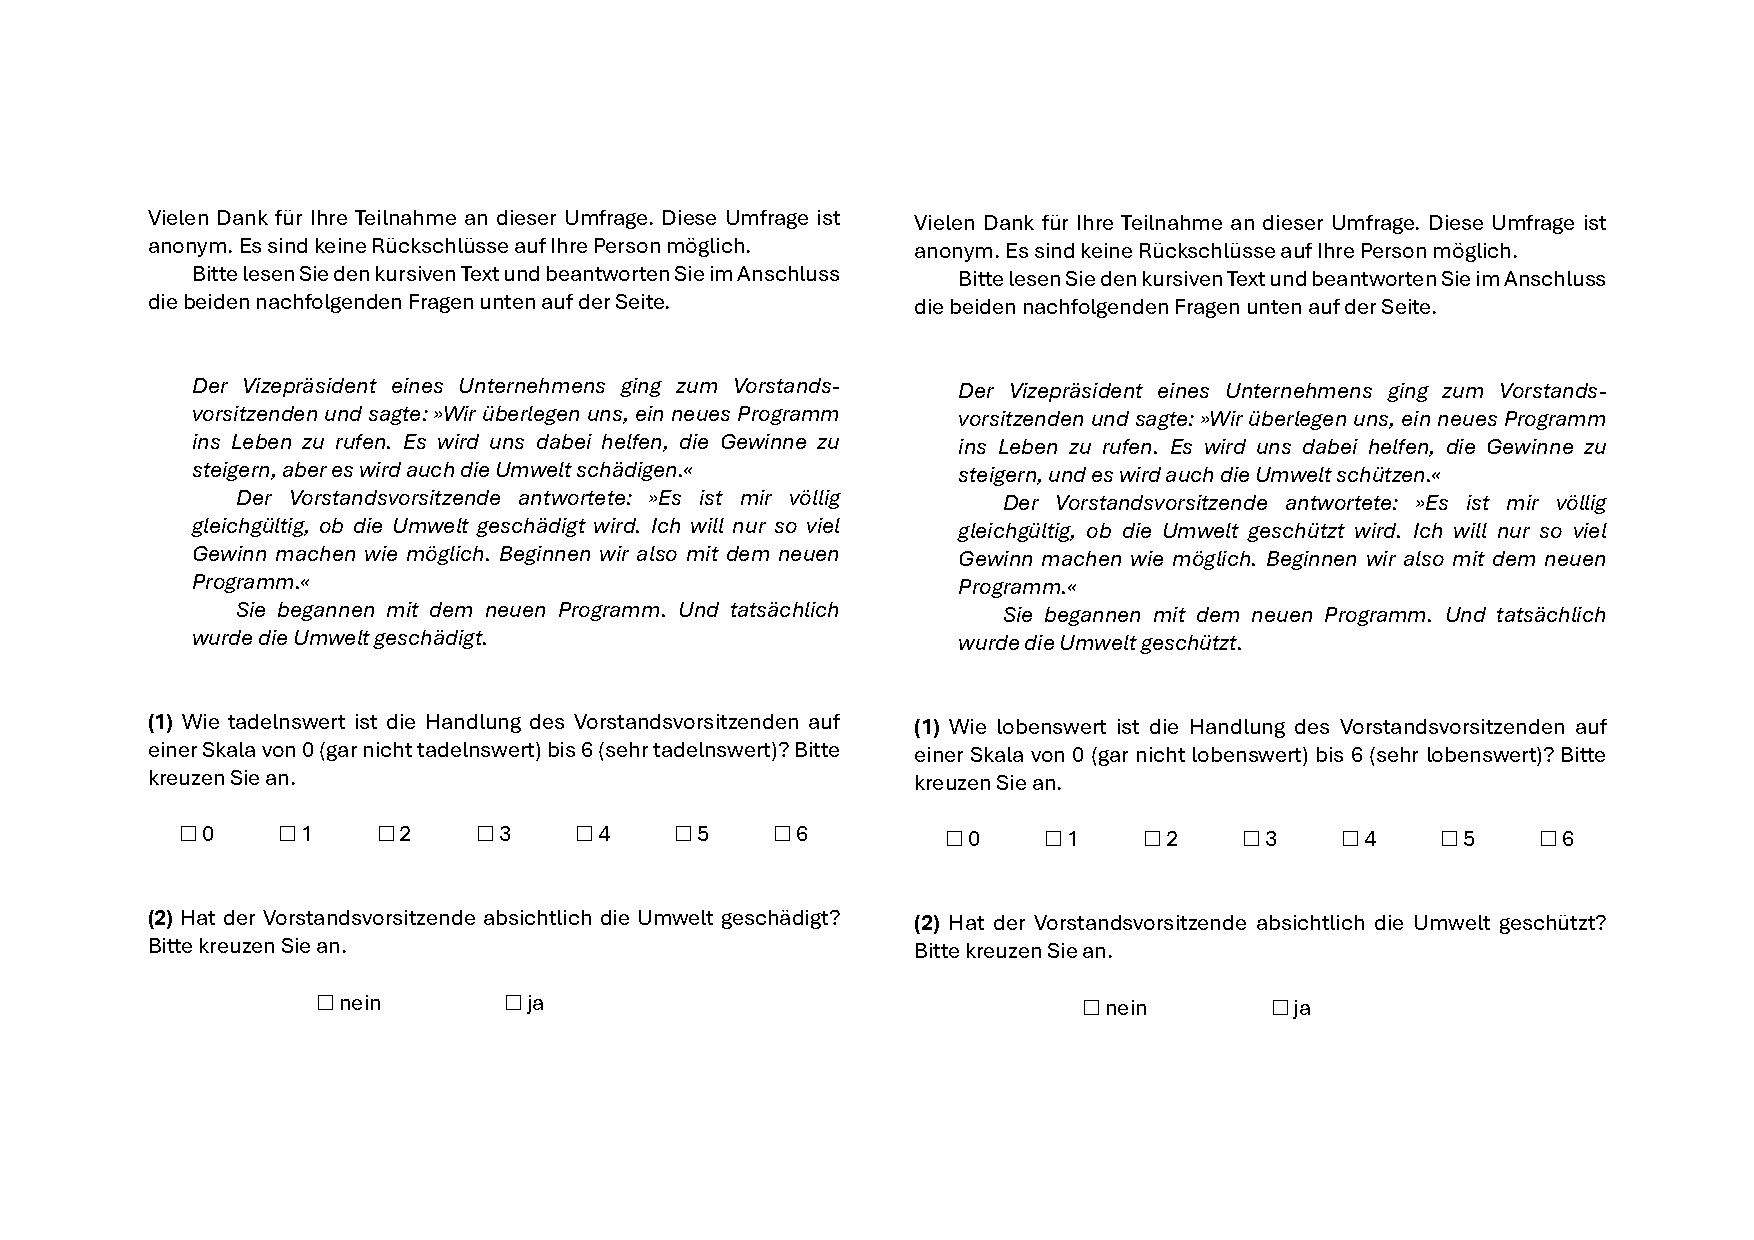
\includegraphics[width=0.5\linewidth]{figures/replication_knobe_survey.pdf}}\\
\end{center}
\end{frame}


%%%%%%%%%%%%%%%%%%%%%%%%%%%%%%%%%%
% FOLIE 16 – ANALYSE REPLIKATION %
%%%%%%%%%%%%%%%%%%%%%%%%%%%%%%%%%%
\begin{frame}
\begin{overlayarea}{\textwidth}{0.81\paperheight}{
   \vspace*{11mm}
   \usebeamerfont{title}\textcolor{uolblue}
   {3\hspace*{1em}Analyse der Replikationsstudie}
}
\end{overlayarea}
\end{frame}


%%%%%%%%%%%%
% FOLIE 17 %
%%%%%%%%%%%%
\begin{frame}{\vspace*{10mm}3\hspace*{1em}Analyse der Replikationsstudie}
\textbf{Datengrundlage}\\
\smallskip
\begin{tabular}[h]{cccc}
   \arrayrulecolor{blue2}\hline
   Person     & Gruppe     & Zuschreibung   & Absicht    \\
   \hline
   1          & B          & 2              & n          \\
   2          & A          & 5              & y          \\
   3          & A          & 4              & y          \\
   $\vdots$   & $\vdots$   & $\vdots$       & $\vdots$   \\
   \hline
\end{tabular}

\bigskip
\textbf{Skalenniveaus}\\
\begin{itemize}
   \item Zuschreibung: ordinal
   \item Absicht: nominal
\end{itemize}

\bigskip
\textcolor{gray}{Die Analyse folgt Bauer, Kornmesser und Meyer (i.\,V.); siehe exemplarisch auch Kuckartz et al. (2013, S.~87\,ff.) und Boslaugh (2012, S.~121\,ff.)}

\note{
   \begin{itemize}
      \item Analyse nominaler Daten über Häufigkeiten
   \end{itemize}
}
\end{frame}


%%%%%%%%%%%%
% FOLIE 18 %
%%%%%%%%%%%%
\begin{frame}{\vspace*{10mm}3\hspace*{1em}Analyse der Replikationsstudie}
\textbf{Beobachtete Häufigkeiten}\\
\smallskip
$f_{o}(\text{Ja}|\text{Schaden})=a$\\
$f_{o}(\text{Ja}|\text{Schützen})=b$\\
$f_{o}(\text{Nein}|\text{Schaden})=c$\\
$f_{o}(\text{Nein}|\text{Schützen})=d$\\

\bigskip
\begin{tabular}{llccc}
   \arrayrulecolor{blue2}\hline
                              &        & \multicolumn{2}{c}{Gruppe}   & Zeilensumme   \\
                              &        & Schaden   & Schützen         &               \\
   \hline
   \multirow{2}{*}{Absicht}   & Ja     & $a$       & $b$              & $a+b$         \\
                              & Nein   & $c$       & $d$              & $c+d$         \\
   \hline
   Spaltensumme               &        & $a+c$     & $b+d$            & $a+b+c+d=n$   \\
   \hline
\end{tabular}
\end{frame}


%%%%%%%%%%%%
% FOLIE 19 %
%%%%%%%%%%%%
\begin{frame}{\vspace*{10mm}3\hspace*{1em}Analyse der Replikationsstudie}
\textbf{Beobachtete Häufigkeiten für Knobe (2003)}\\
\smallskip
Unter der Annahme, dass die 78 Personen gleich auf beide Gruppen aufgeteilt sind:\\
\smallskip
$f_{o}(\text{Ja}|\text{Schaden})=32$\hspace{2em}$\leftarrow$ \enquote{most subjects (82\%)} \textcolor{gray}{(Knobe 2003, S.~192)}\\
$f_{o}(\text{Ja}|\text{Schützen})=9$\\
$f_{o}(\text{Nein}|\text{Schaden})=7$\\
$f_{o}(\text{Nein}|\text{Schützen})=30$\hspace{2em}$\leftarrow$ \enquote{most subjects (77\%)} \textcolor{gray}{(ebd.)}\\

\bigskip
\begin{tabular}{llccc}
   \arrayrulecolor{blue2}\hline
                              &        & \multicolumn{2}{c}{Gruppe}   & Zeilensumme   \\
                              &        & Schaden   & Schützen         &               \\
   \hline
   \multirow{2}{*}{Absicht}   & Ja     & 32        &  9               & 41            \\
                              & Nein   &  7        & 30               & 37            \\
   \hline
   Spaltensumme               &        & 39        & 39               & 78            \\
   \hline
\end{tabular}
\end{frame}


%%%%%%%%%%%%
% FOLIE 20 %
%%%%%%%%%%%%
\begin{frame}{\vspace*{10mm}3\hspace*{1em}Analyse der Replikationsstudie}
\textbf{Nullhypothese (H$_{0}$)}\\
\smallskip
Die Antworten auf die Frage, ob der Vorsitzende die Umwelt absichtlich geschädigt oder geschützt hat, sind unabhängig von der Gruppe.\\
\smallskip
$P(\text{Absicht}|\text{Gruppe})=P(\text{Absicht})$\\

\bigskip
\textbf{Alternativhypothese (H$_{1}$)}\\
\smallskip
Die Antworten auf die Frage, ob der Vorsitzende die Umwelt absichtlich geschädigt oder geschützt hat, sind abhängig von der Gruppe.\\
\smallskip
$P(\text{Absicht}|\text{Gruppe})\neq P(\text{Absicht})$\\
\end{frame}


%%%%%%%%%%%%
% FOLIE 21 %
%%%%%%%%%%%%
\begin{frame}{\vspace*{10mm}3\hspace*{1em}Analyse der Replikationsstudie}
\textbf{Erwartete Wahrscheinlichkeit bei Unabhängigkeit}\\
\smallskip
$P(\text{Absicht}|\text{Gruppe})=P(\text{Absicht})$\\

\bigskip
\textbf{Erwartete Wahrscheinlichkeit bei Unabhängigkeit für Antworten}\\
\smallskip
$P(\text{Ja})=\dfrac{\text{Zeilensumme (Ja)}}{\text{Teilnehmer}}$\\
\medskip
$P(\text{Nein})=\dfrac{\text{Zeilensumme (Nein)}}{\text{Teilnehmer}}$\\

\bigskip
\textbf{Erwartete Häufigkeit bei Unabhängigkeit für einzelne Zelle}\\
\smallskip
$f_{e}(\text{Zelle})=\dfrac{\text{Spaltensumme}\times\text{Zeilensumme}}{\text{Teilnehmer}}$\\
\end{frame}


%%%%%%%%%%%%
% FOLIE 22 %
%%%%%%%%%%%%
\begin{frame}{\vspace*{10mm}3\hspace*{1em}Analyse der Replikationsstudie}
\textbf{Erwartete Häufigkeiten bei Unabhängigkeit für Knobe (2003)}\\
\smallskip
$f_{e}(\text{Ja}|\text{Schaden})=\dfrac{39\times41}{78}=20,5$\\
\smallskip
$f_{e}(\text{Ja}|\text{Schützen})=\dfrac{39\times41}{78}=20,5$\\
\smallskip
$f_{e}(\text{Nein}|\text{Schaden})=\dfrac{39\times37}{78}=18,5$\\
\smallskip
$f_{e}(\text{Nein}|\text{Schützen})=\dfrac{39\times37}{78}=18,5$\\

\bigskip
\begin{tabular}{llcc}
   \arrayrulecolor{blue2}\hline
                              &        & \multicolumn{2}{c}{Gruppe}   \\
                              &        & Schaden   & Schützen         \\
   \hline
   \multirow{2}{*}{Absicht}   & Ja     & 20,5      & 20,5             \\
                              & Nein   & 18,5      & 18,5             \\
   \hline
\end{tabular}
\end{frame}


%%%%%%%%%%%%
% FOLIE 23 %
%%%%%%%%%%%%
\begin{frame}{\vspace*{10mm}3\hspace*{1em}Analyse der Replikationsstudie}
\textbf{Berechnung der Residuen}\\
\smallskip
\begin{tabular}{llcc}
   \arrayrulecolor{blue2}\hline
                              &        & \multicolumn{2}{c}{Gruppe}                    \\
                              &        & Schaden               & Schützen              \\
   \hline
   \multirow{2}{*}{Absicht}   & Ja     & $f_{o}(a)-f_{e}(a)$   & $f_{o}(b)-f_{e}(b)$   \\
                              & Nein   & $f_{o}(c)-f_{e}(c)$   & $f_{o}(d)-f_{e}(d)$   \\
   \hline
\end{tabular}
\end{frame}


%%%%%%%%%%%%
% FOLIE 24 %
%%%%%%%%%%%%
\begin{frame}{\vspace*{10mm}3\hspace*{1em}Analyse der Replikationsstudie}
\textbf{Berechnung der Residuen für Knobe (2003)}\\
\smallskip
\begin{tabular}{llcc}
   \arrayrulecolor{blue2}\hline
                              &        & \multicolumn{2}{c}{Gruppe}          \\
                              &        & Schaden          & Schützen         \\
   \hline
   \multirow{2}{*}{Absicht}   & Ja     & $32-20,5=11,5$   & $9-20,5=-11,5$   \\
                              & Nein   & $7-18,5=-11,5$   & $30-18,5=11,5$   \\
   \hline
\end{tabular}
\end{frame}


%%%%%%%%%%%%
% FOLIE 25 %
%%%%%%%%%%%%
\begin{frame}{\vspace*{10mm}3\hspace*{1em}Analyse der Replikationsstudie}
\textbf{Berechnung der $\chi^{2}$-Statistik}\\
\smallskip
$\chi^{2}=\sum_{z=1}^{4}\dfrac{(f_{o}(z)-f_{e}(z))^{2}}{f_{e}(z)}$
\end{frame}


%%%%%%%%%%%%
% FOLIE 26 %
%%%%%%%%%%%%
\begin{frame}{\vspace*{10mm}3\hspace*{1em}Analyse der Replikationsstudie}
\textbf{Berechnung der $\chi^{2}$-Statistik für Knobe (2003)}\\
\smallskip
$\chi^{2}=\dfrac{(32-20,5)^{2}}{20,5}+\dfrac{(9-20,5)^{2}}{20,5}+\dfrac{(7-18,5)^{2}}{18,5}+\dfrac{(30-18,5)^{2}}{18,5}\approx27,2$

\bigskip
Zum Vergleich: \enquote{$\chi^{2}(1,N=78)=27.2$} \textcolor{gray}{(Knobe 2003, S.~192)}
\end{frame}


%%%%%%%%%%%%
% FOLIE 27 %
%%%%%%%%%%%%
\begin{frame}{\vspace*{10mm}3\hspace*{1em}Analyse der Replikationsstudie}
\textbf{$\chi^{2}$-Verteilung}\\
\begin{center}
   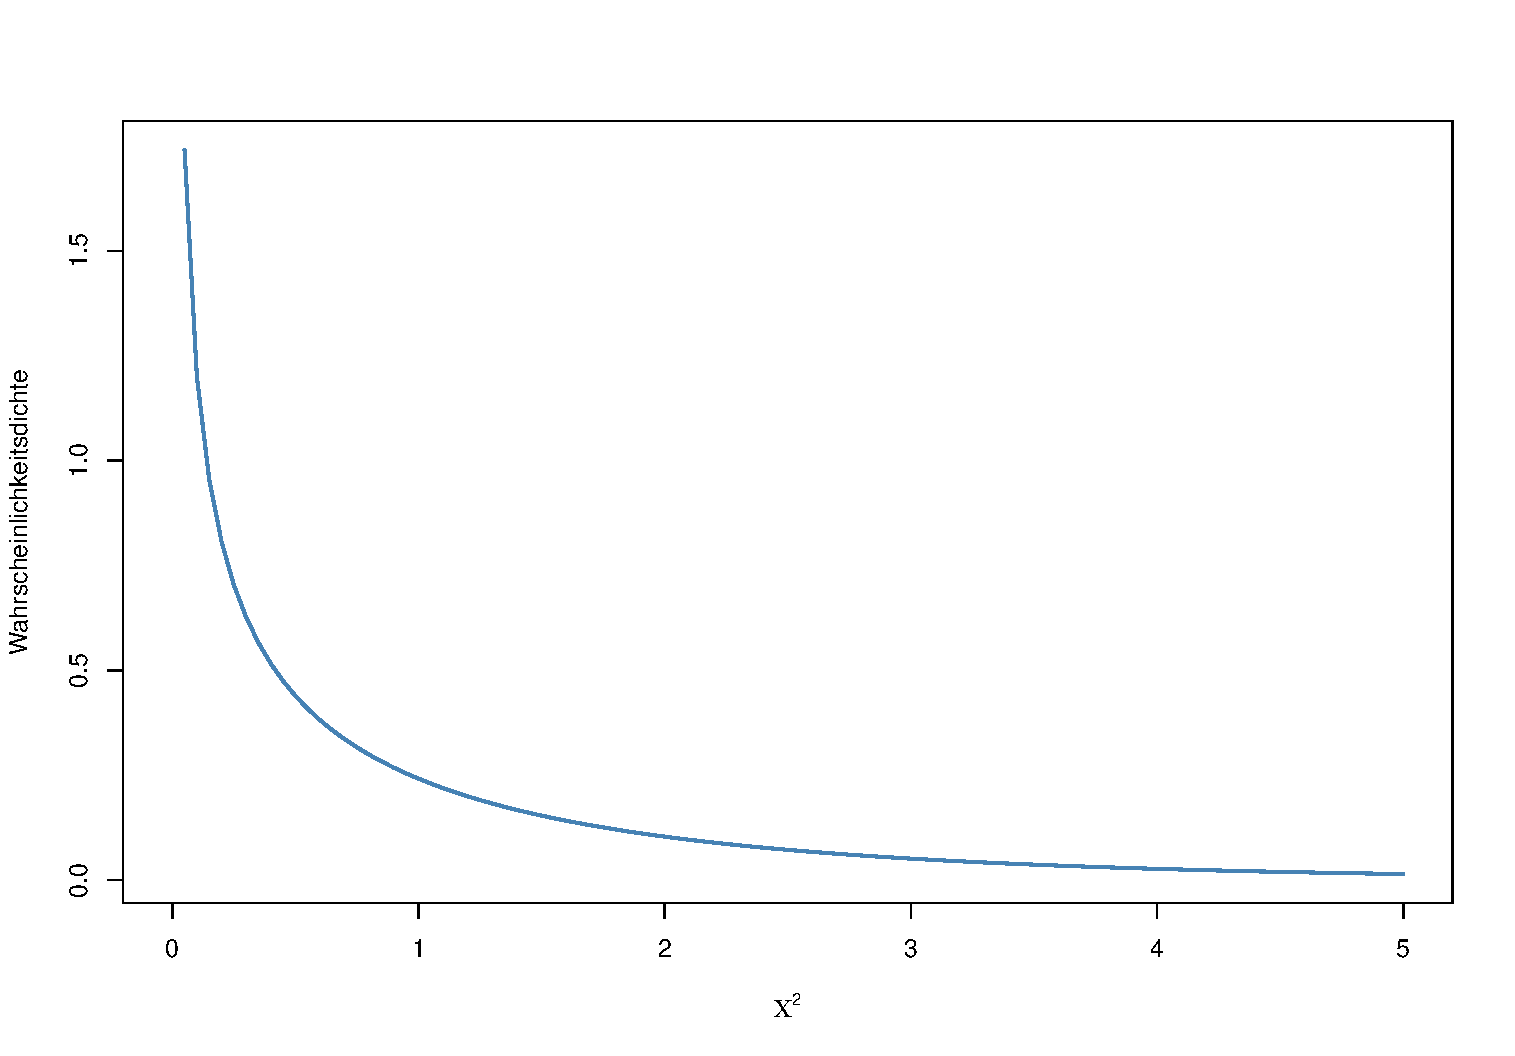
\includegraphics[width=0.5\linewidth]{figures/replication_knobe_distribution.pdf}\\
   \textcolor{gray}{$\chi^{2}$-Verteilung ($df=1$)}
\end{center}

\note{
   \begin{itemize}
      \item Wahrscheinlichkeitsdichtefunktion für den Fall, dass Unabhängigkeit vorliegt
      \item Wahrscheinlichkeit, dass ein gewisser $\chi^{2}$-Wert innerhalb eines Intervalls auf der x-Achse liegt
      \item Festlegung von Annahme- oder Akzeptanzbereich durch Testniveau $\alpha$
   \end{itemize}
}
\end{frame}


%%%%%%%%%%%%
% FOLIE 28 %
%%%%%%%%%%%%
\begin{frame}{\vspace*{10mm}3\hspace*{1em}Analyse der Replikationsstudie}
\textbf{Signifikanzniveau}\\
\smallskip
$\alpha=0,05$ (kritischer $\chi^{2}$-Wert: 3,84)\\
\smallskip
$\alpha=0,001$ (kritischer $\chi^{2}$-Wert: 10,83)

\bigskip
Zum Vergleich: \enquote{This difference was highly statistically significant [$\ldots$], $p<.001$}\\
\textcolor{gray}{(Knobe 2003, S.~192)}

\note{
   \begin{itemize}
      \item Wie hoch die Wahrscheinlichkeit sein soll, die Nullhypothese zu verwerfen, obwohl sie eigentlich zutrifft
      \item Gilt die Nullhypothese, nimmt die $\chi^{2}$-Statistik mit einer Wahrscheinlichkeit von $95\%$ einen Wert zwischen 0 und 3,841 an; mit einer Wahrscheinlichkeit von $5\%$ ist der Wert größer als 3,841
   \end{itemize}
}
\end{frame}


%%%%%%%%%%%%
% FOLIE 29 %
%%%%%%%%%%%%
\begin{frame}{\vspace*{10mm}3\hspace*{1em}Analyse der Replikationsstudie}
\textbf{Online-$\chi^{2}$-Rechner}\\
\smallskip
\url{https://datatab.net/}

\bigskip
\begin{center}
   \frame{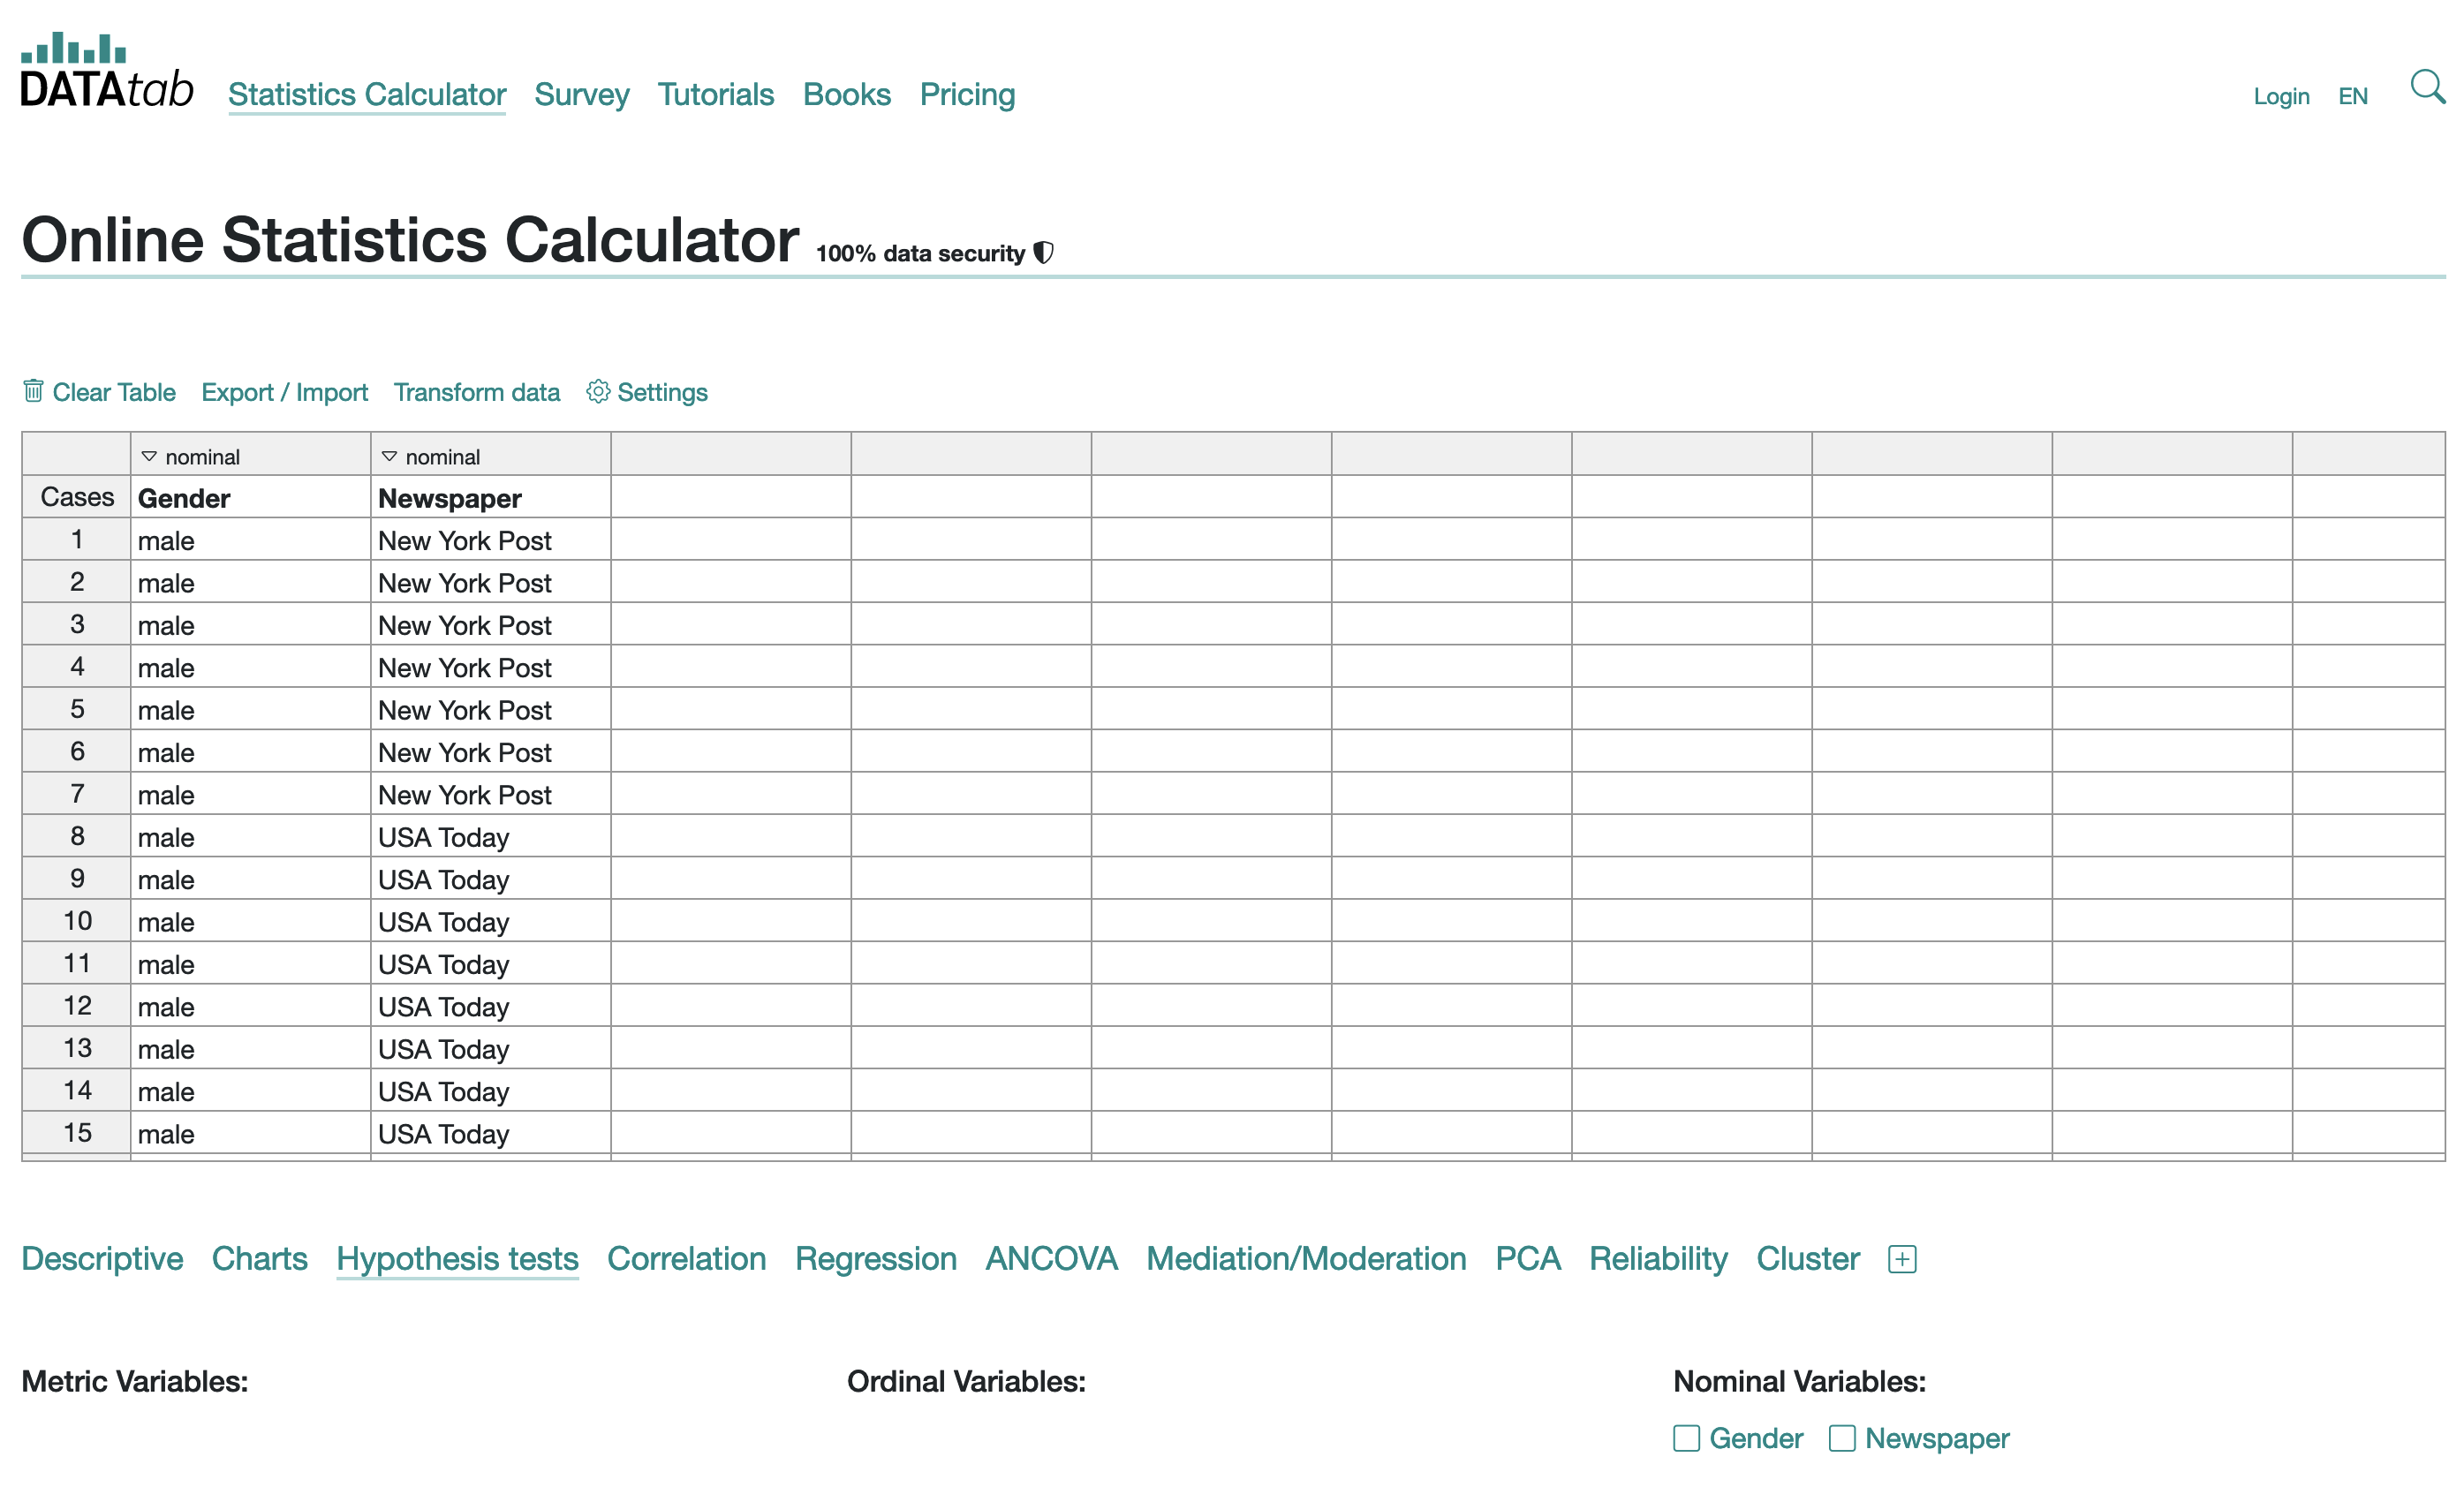
\includegraphics[width=0.55\linewidth]{figures/replication_knobe_calculator.png}}\\
   \textcolor{gray}{DATAtab Team (2024)}
\end{center}
\end{frame}


%%%%%%%%%%%%%%%%%%%%%%%%%%%%%%%%%%%%%
% FOLIE 30 – ERGEBNISSE REPLIKATION %
%%%%%%%%%%%%%%%%%%%%%%%%%%%%%%%%%%%%%
\begin{frame}
\begin{overlayarea}{\textwidth}{0.81\paperheight}{
   \vspace*{11mm}
   \usebeamerfont{title}\textcolor{uolblue}
   {4\hspace*{1em}Ergebnisse der Replikationsstudie}
}
\end{overlayarea}
\end{frame}


%%%%%%%%%%%%
% FOLIE 31 %
%%%%%%%%%%%%
\begin{frame}{\vspace*{10mm}4\hspace*{1em}Ergebnisse der Replikationsstudie}
\textbf{Offene Wissenschaft und offene Daten}\\
\smallskip
\url{https://github.com/alephmembeth/course-x-phi-2024}

\bigskip
\begin{center}
   \frame{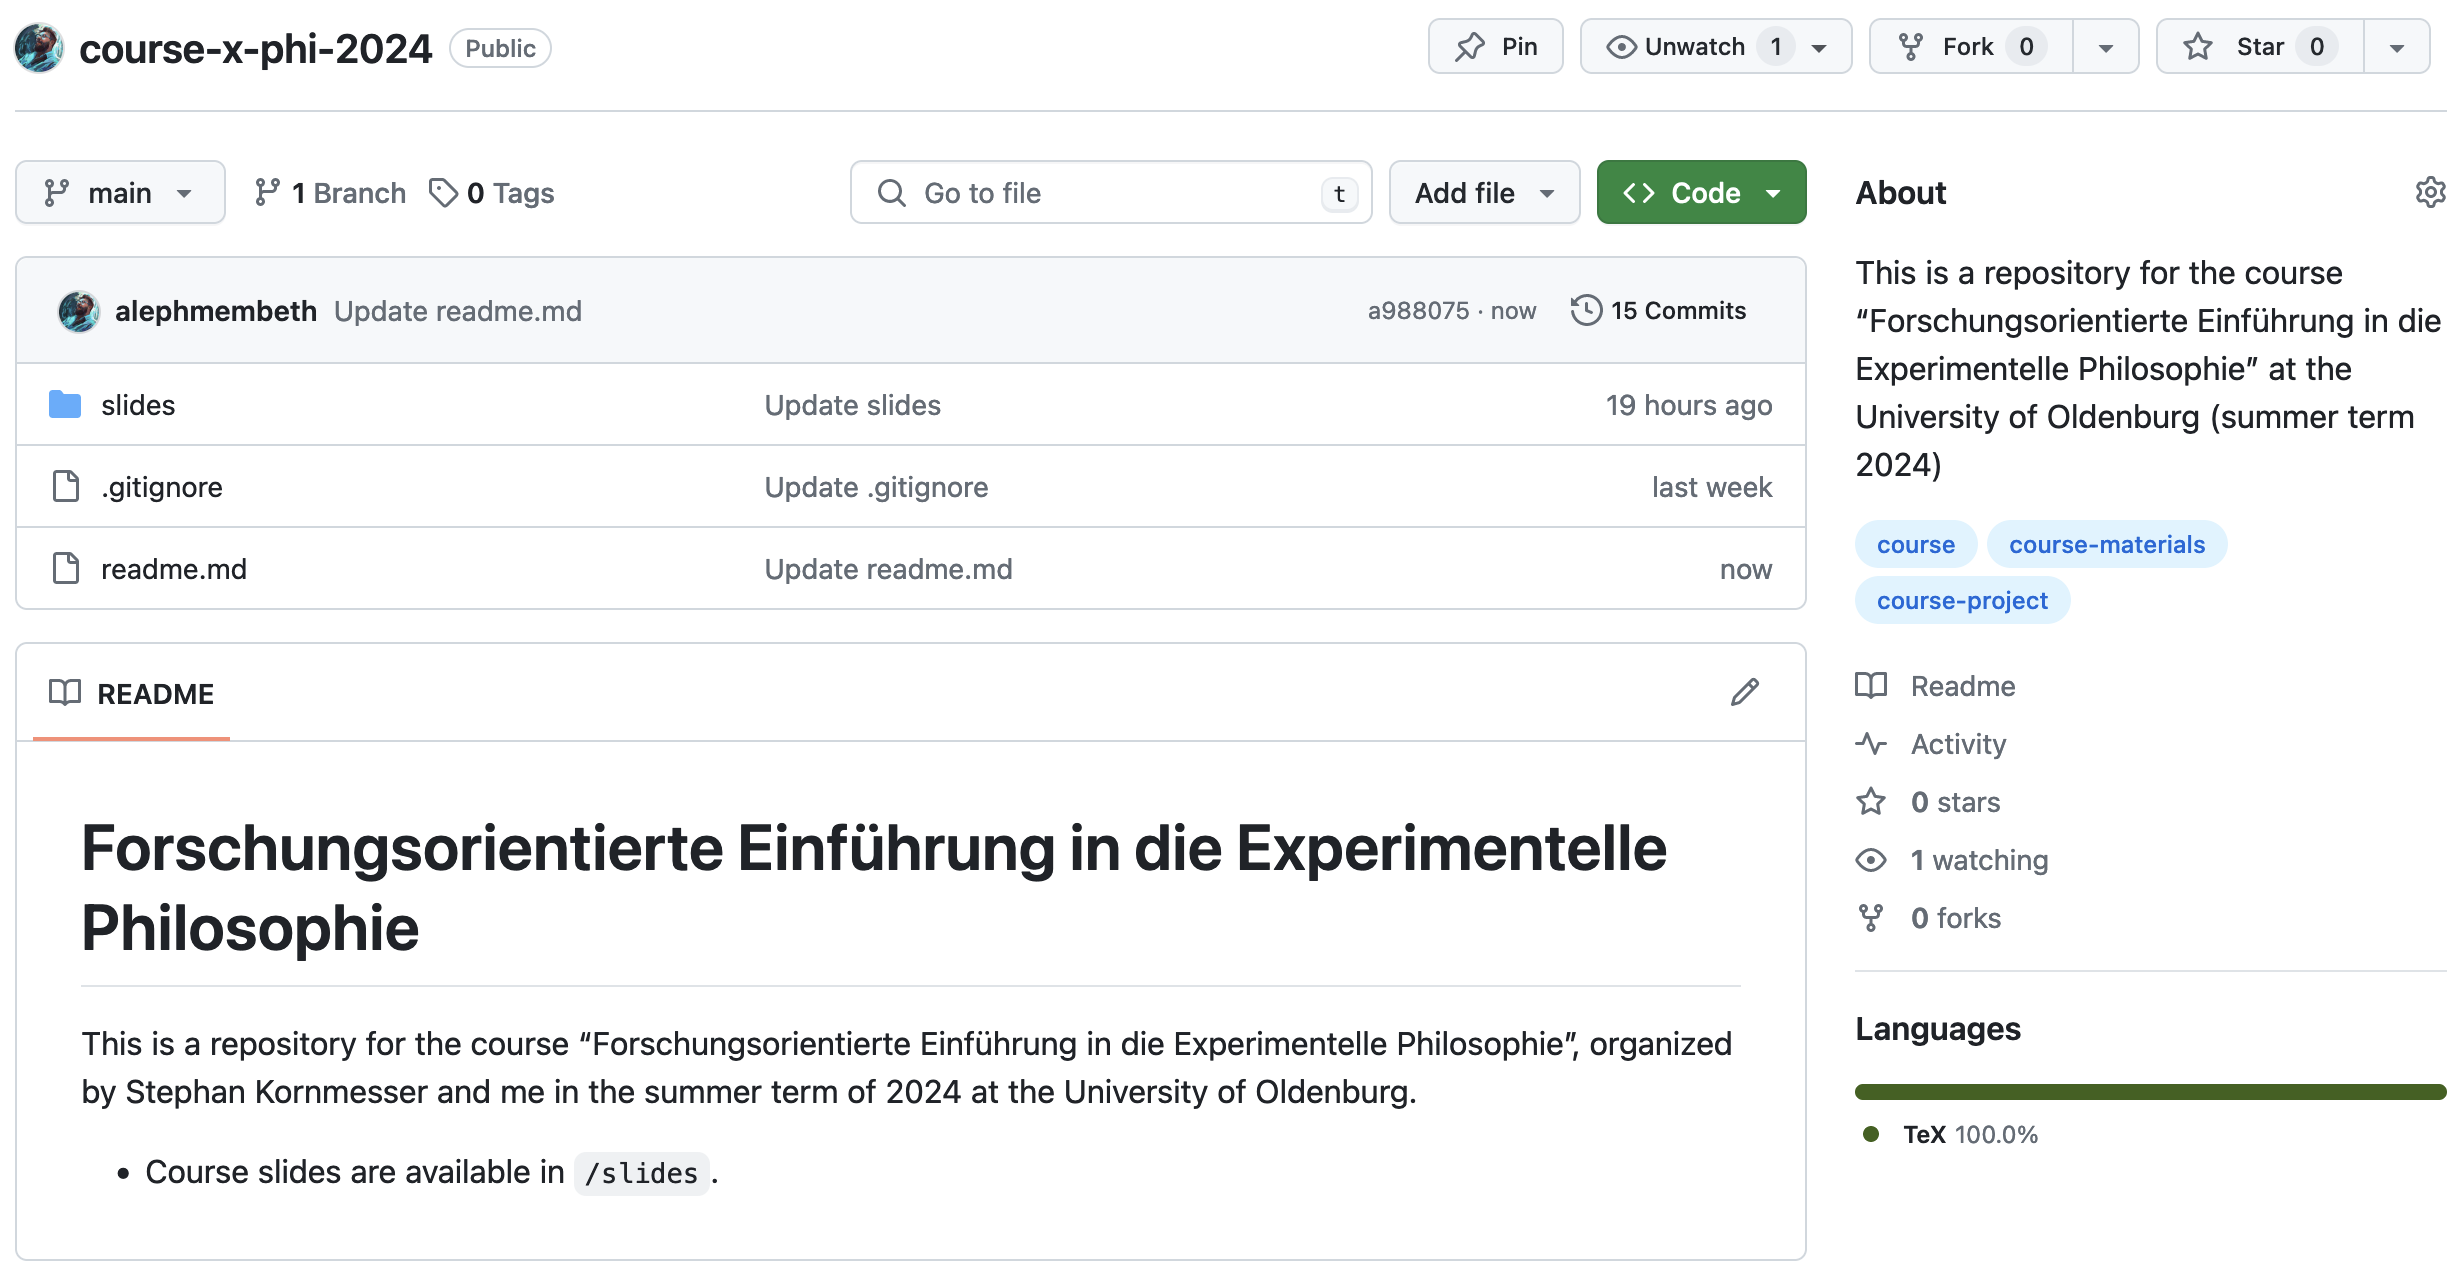
\includegraphics[width=0.55\linewidth]{figures/replication_knobe_github.png}}\\
\end{center}
\end{frame}


%%%%%%%%%%%%
% FOLIE 32 %
%%%%%%%%%%%%
\begin{frame}{\vspace*{10mm}4\hspace*{1em}Ergebnisse der Replikationsstudie}
\textbf{Auswertung mit R (1/4)}\\
\smallskip
\lstset{style=mystyle}
\lstinputlisting[language=R]{code/replication_knobe_part_1.R}
\end{frame}


%%%%%%%%%%%%
% FOLIE 33 %
%%%%%%%%%%%%
\begin{frame}{\vspace*{10mm}4\hspace*{1em}Ergebnisse der Replikationsstudie}
\textbf{Auswertung mit R (2/4)}\\
\smallskip
\lstset{style=mystyle}
\lstinputlisting[language=R]{code/replication_knobe_part_2.R}
\end{frame}


%%%%%%%%%%%%
% FOLIE 34 %
%%%%%%%%%%%%
\begin{frame}{\vspace*{10mm}4\hspace*{1em}Ergebnisse der Replikationsstudie}
\textbf{Auswertung mit R (3/4)}\\
\smallskip
\lstset{style=mystyle}
\lstinputlisting[language=R]{code/replication_knobe_part_3.R}
\end{frame}


%%%%%%%%%%%%
% FOLIE 35 %
%%%%%%%%%%%%
\begin{frame}{\vspace*{10mm}4\hspace*{1em}Ergebnisse der Replikationsstudie}
\textbf{Auswertung mit R (4/4)}\\
\smallskip
\lstset{style=mystyle}
\lstinputlisting[language=R]{code/replication_knobe_part_4.R}
\end{frame}


%%%%%%%%%%%%
% FOLIE 36 %
%%%%%%%%%%%%
\begin{frame}{\vspace*{10mm}4\hspace*{1em}Ergebnisse der Replikationsstudie}
\textbf{Ergebnisse Gruppe 1}\\
\begin{multicols}{2}
   \begin{center}
      \frame{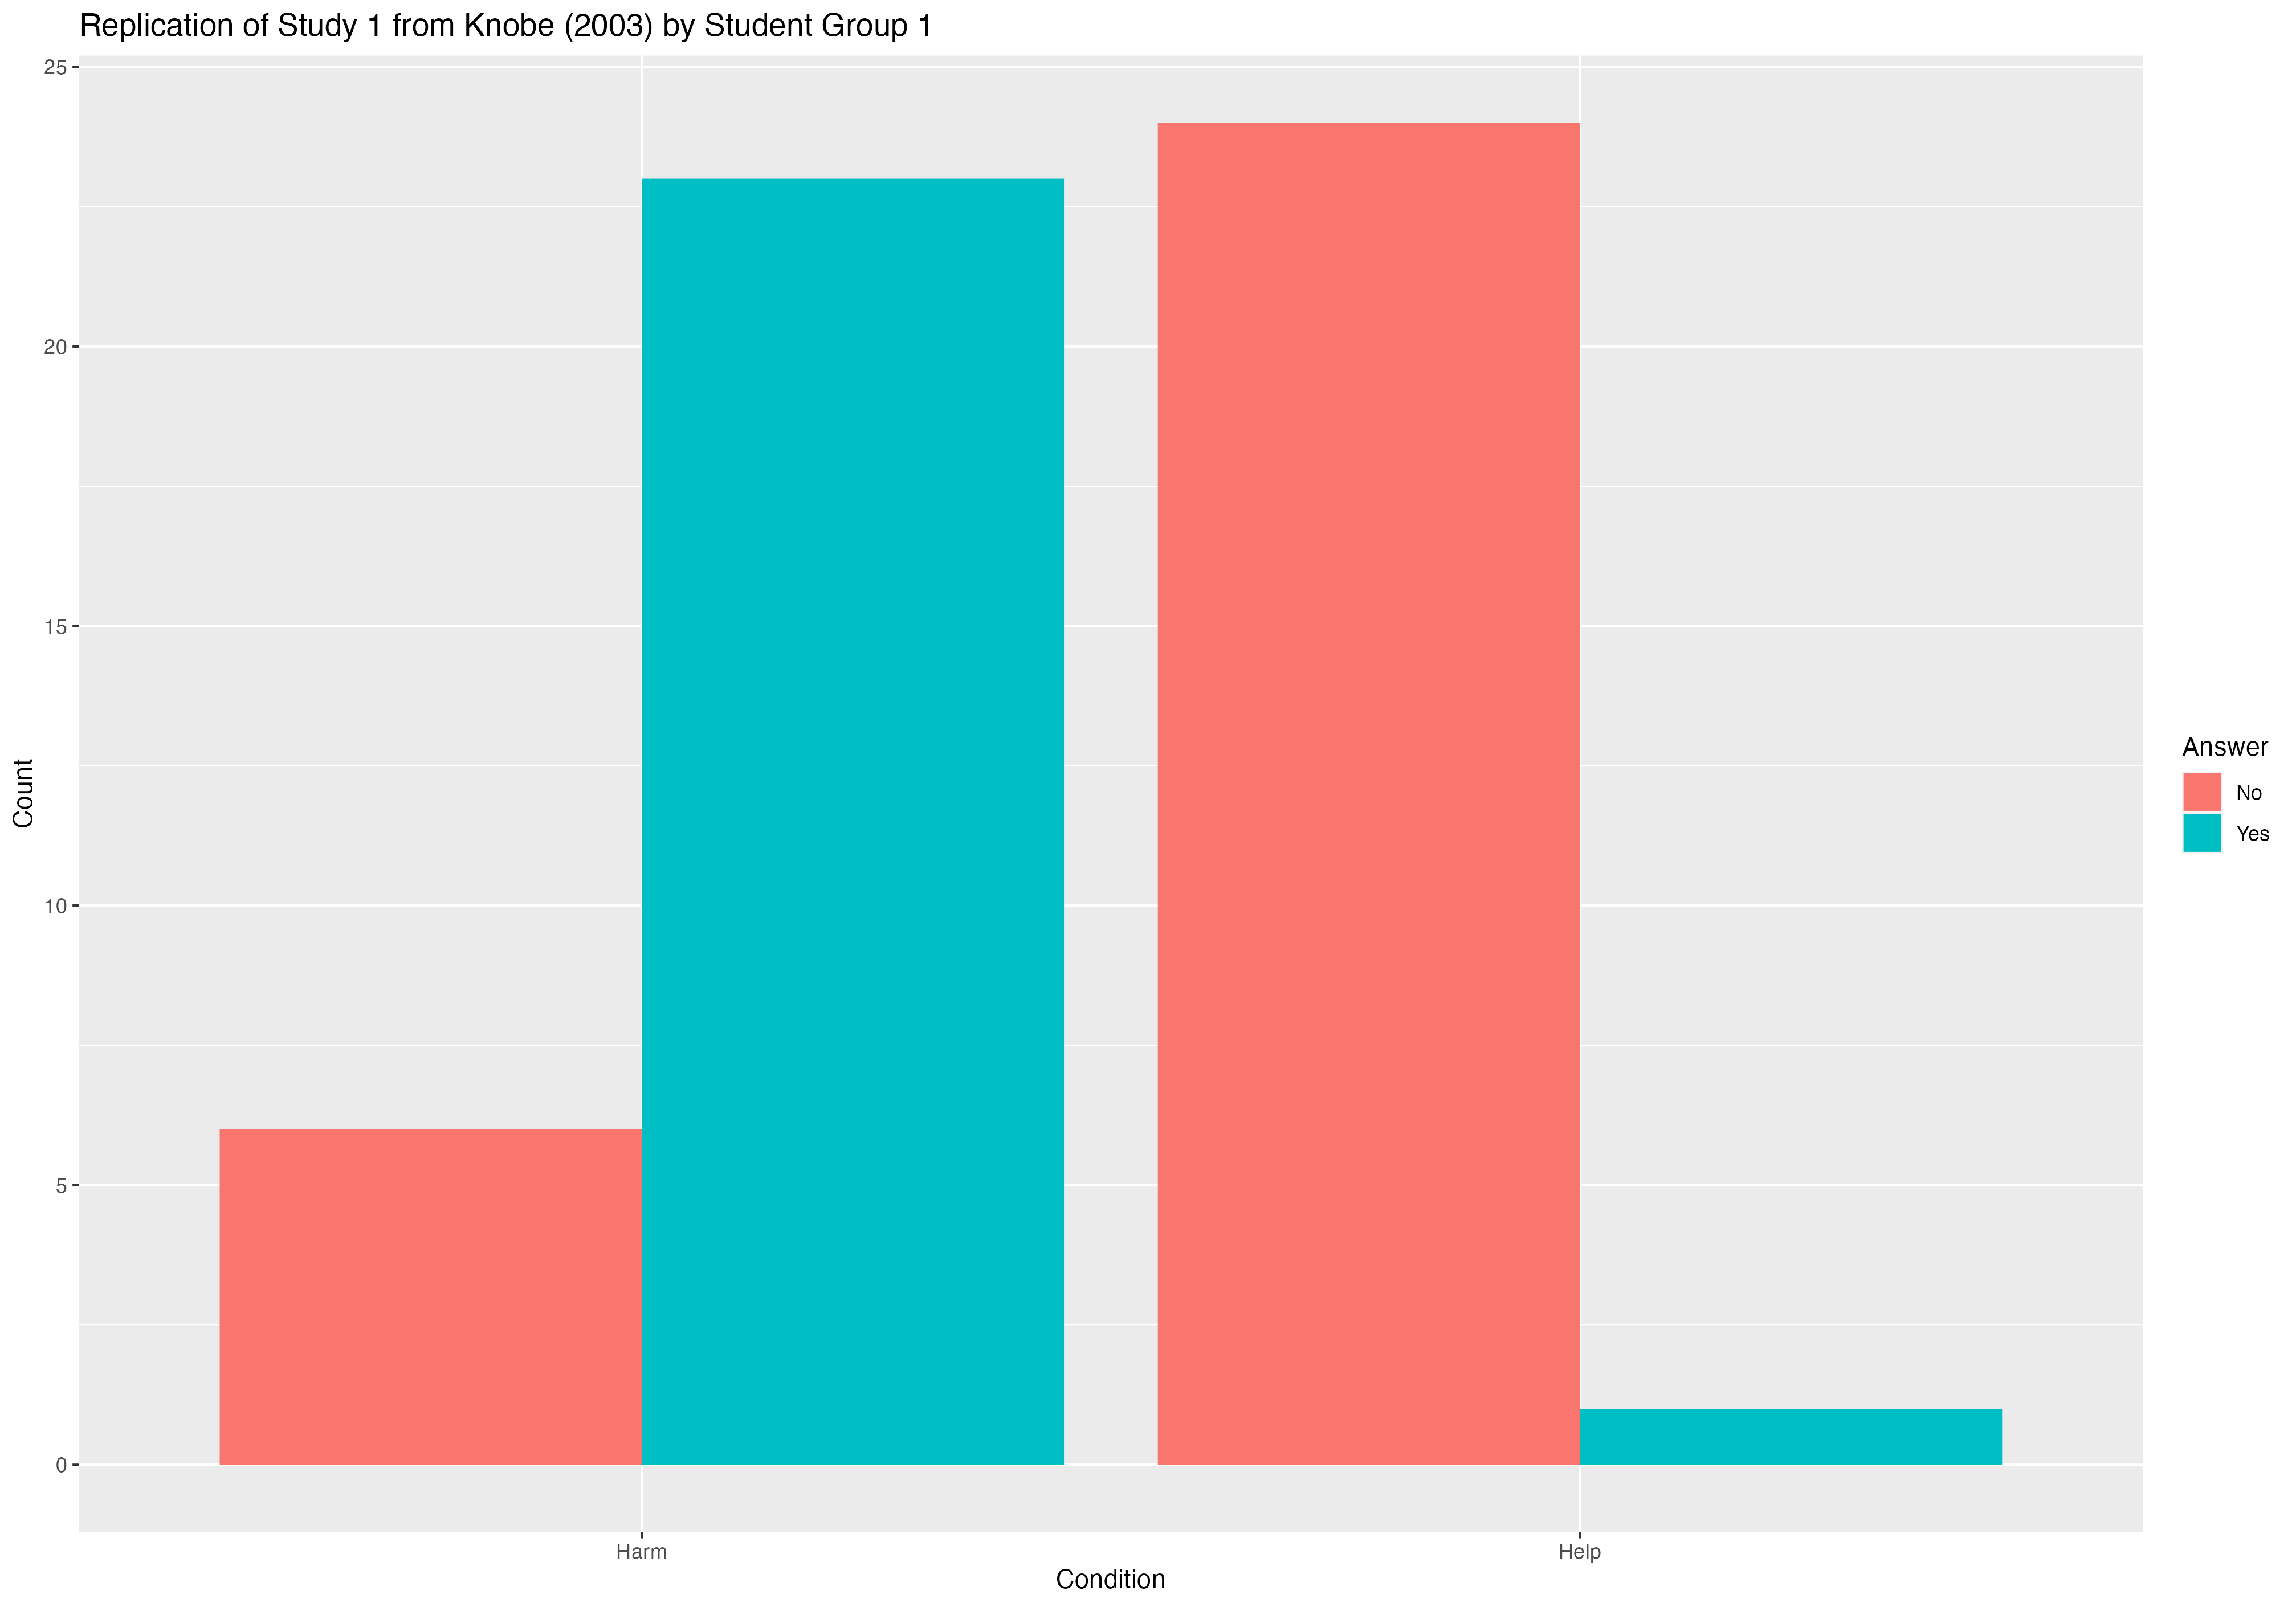
\includegraphics[width=0.75\linewidth]{figures/replication_knobe_fig_1.png}}\\
      \frame{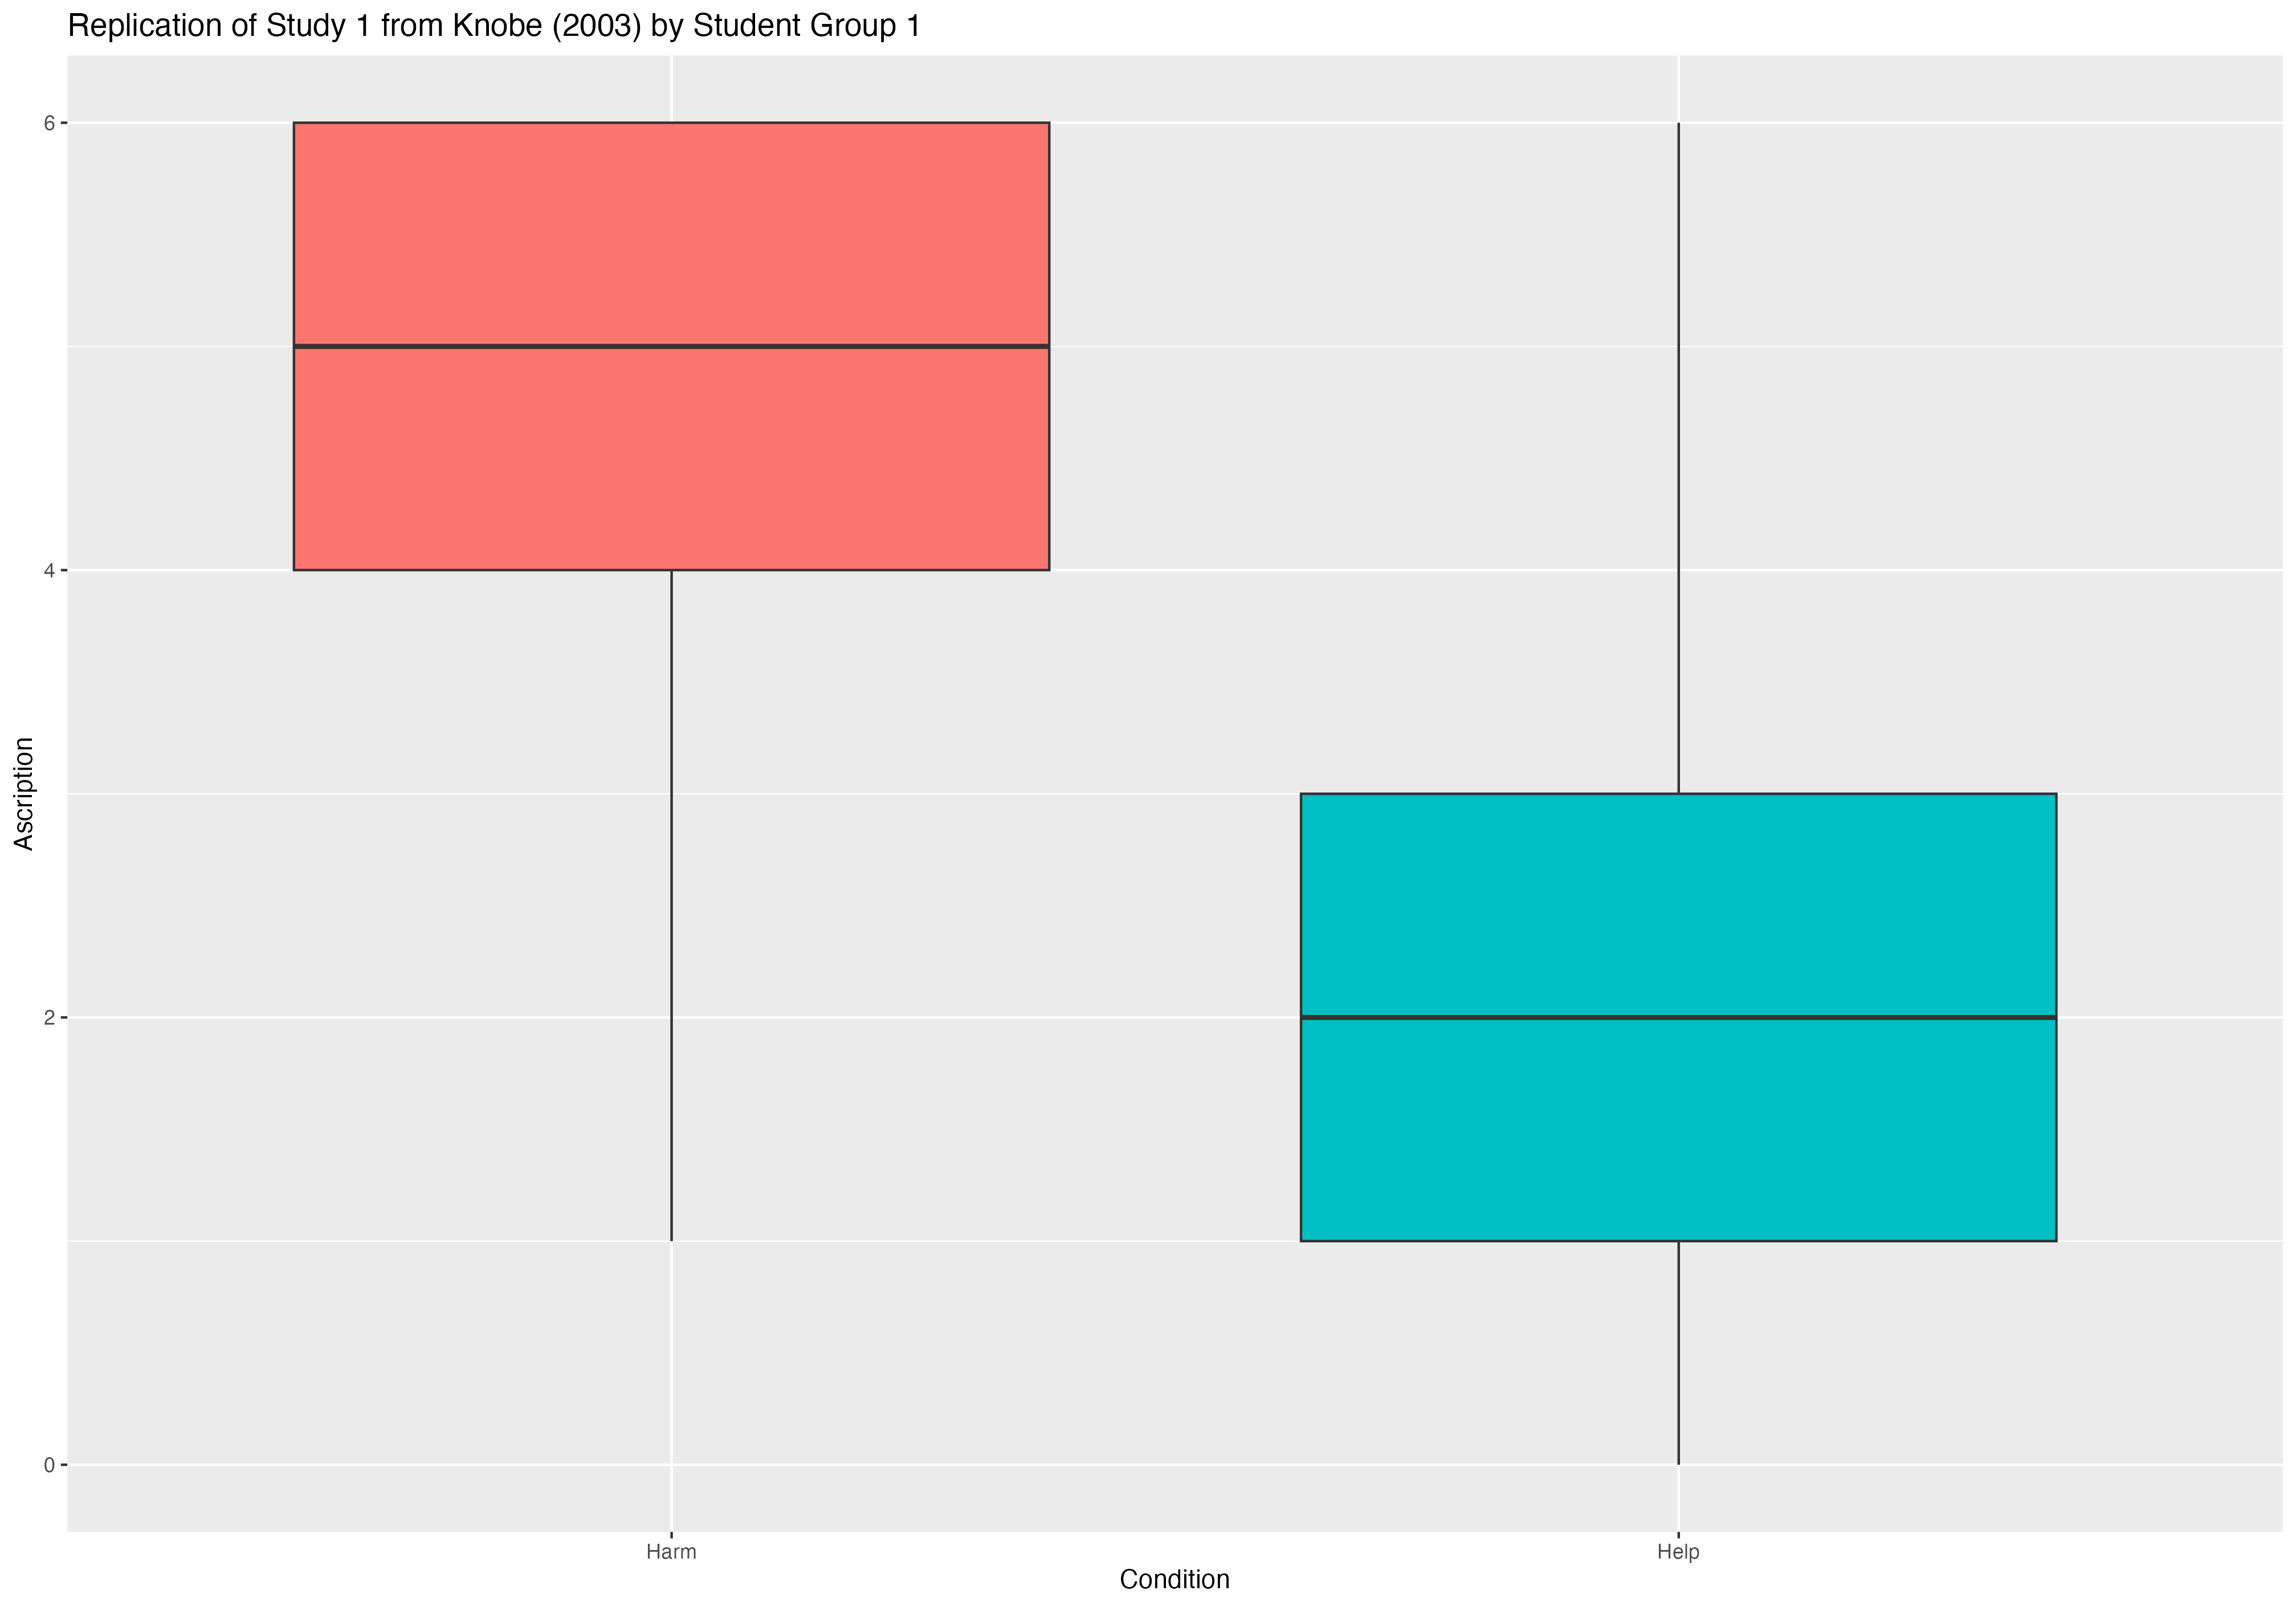
\includegraphics[width=0.75\linewidth]{figures/replication_knobe_fig_2.png}}\\
   \end{center}
\end{multicols}
\textbf{Antwort:} $\chi^2(df=1,n=54)=27,865$, $p<0,001$; $w=0,756$\\

\medskip
\textbf{Zuschreibung:} Schaden $M=4,90$, $SD=1,26$; Helfen $M=2,32$, $SD=1,63$; $t=6,43$, $p<0,001$; $d=1,77$
\end{frame}


%%%%%%%%%%%%
% FOLIE 37 %
%%%%%%%%%%%%
\begin{frame}{\vspace*{10mm}4\hspace*{1em}Ergebnisse der Replikationsstudie}
\textbf{Ergebnisse Gruppe 2}\\
\begin{multicols}{2}
   \begin{center}
      \frame{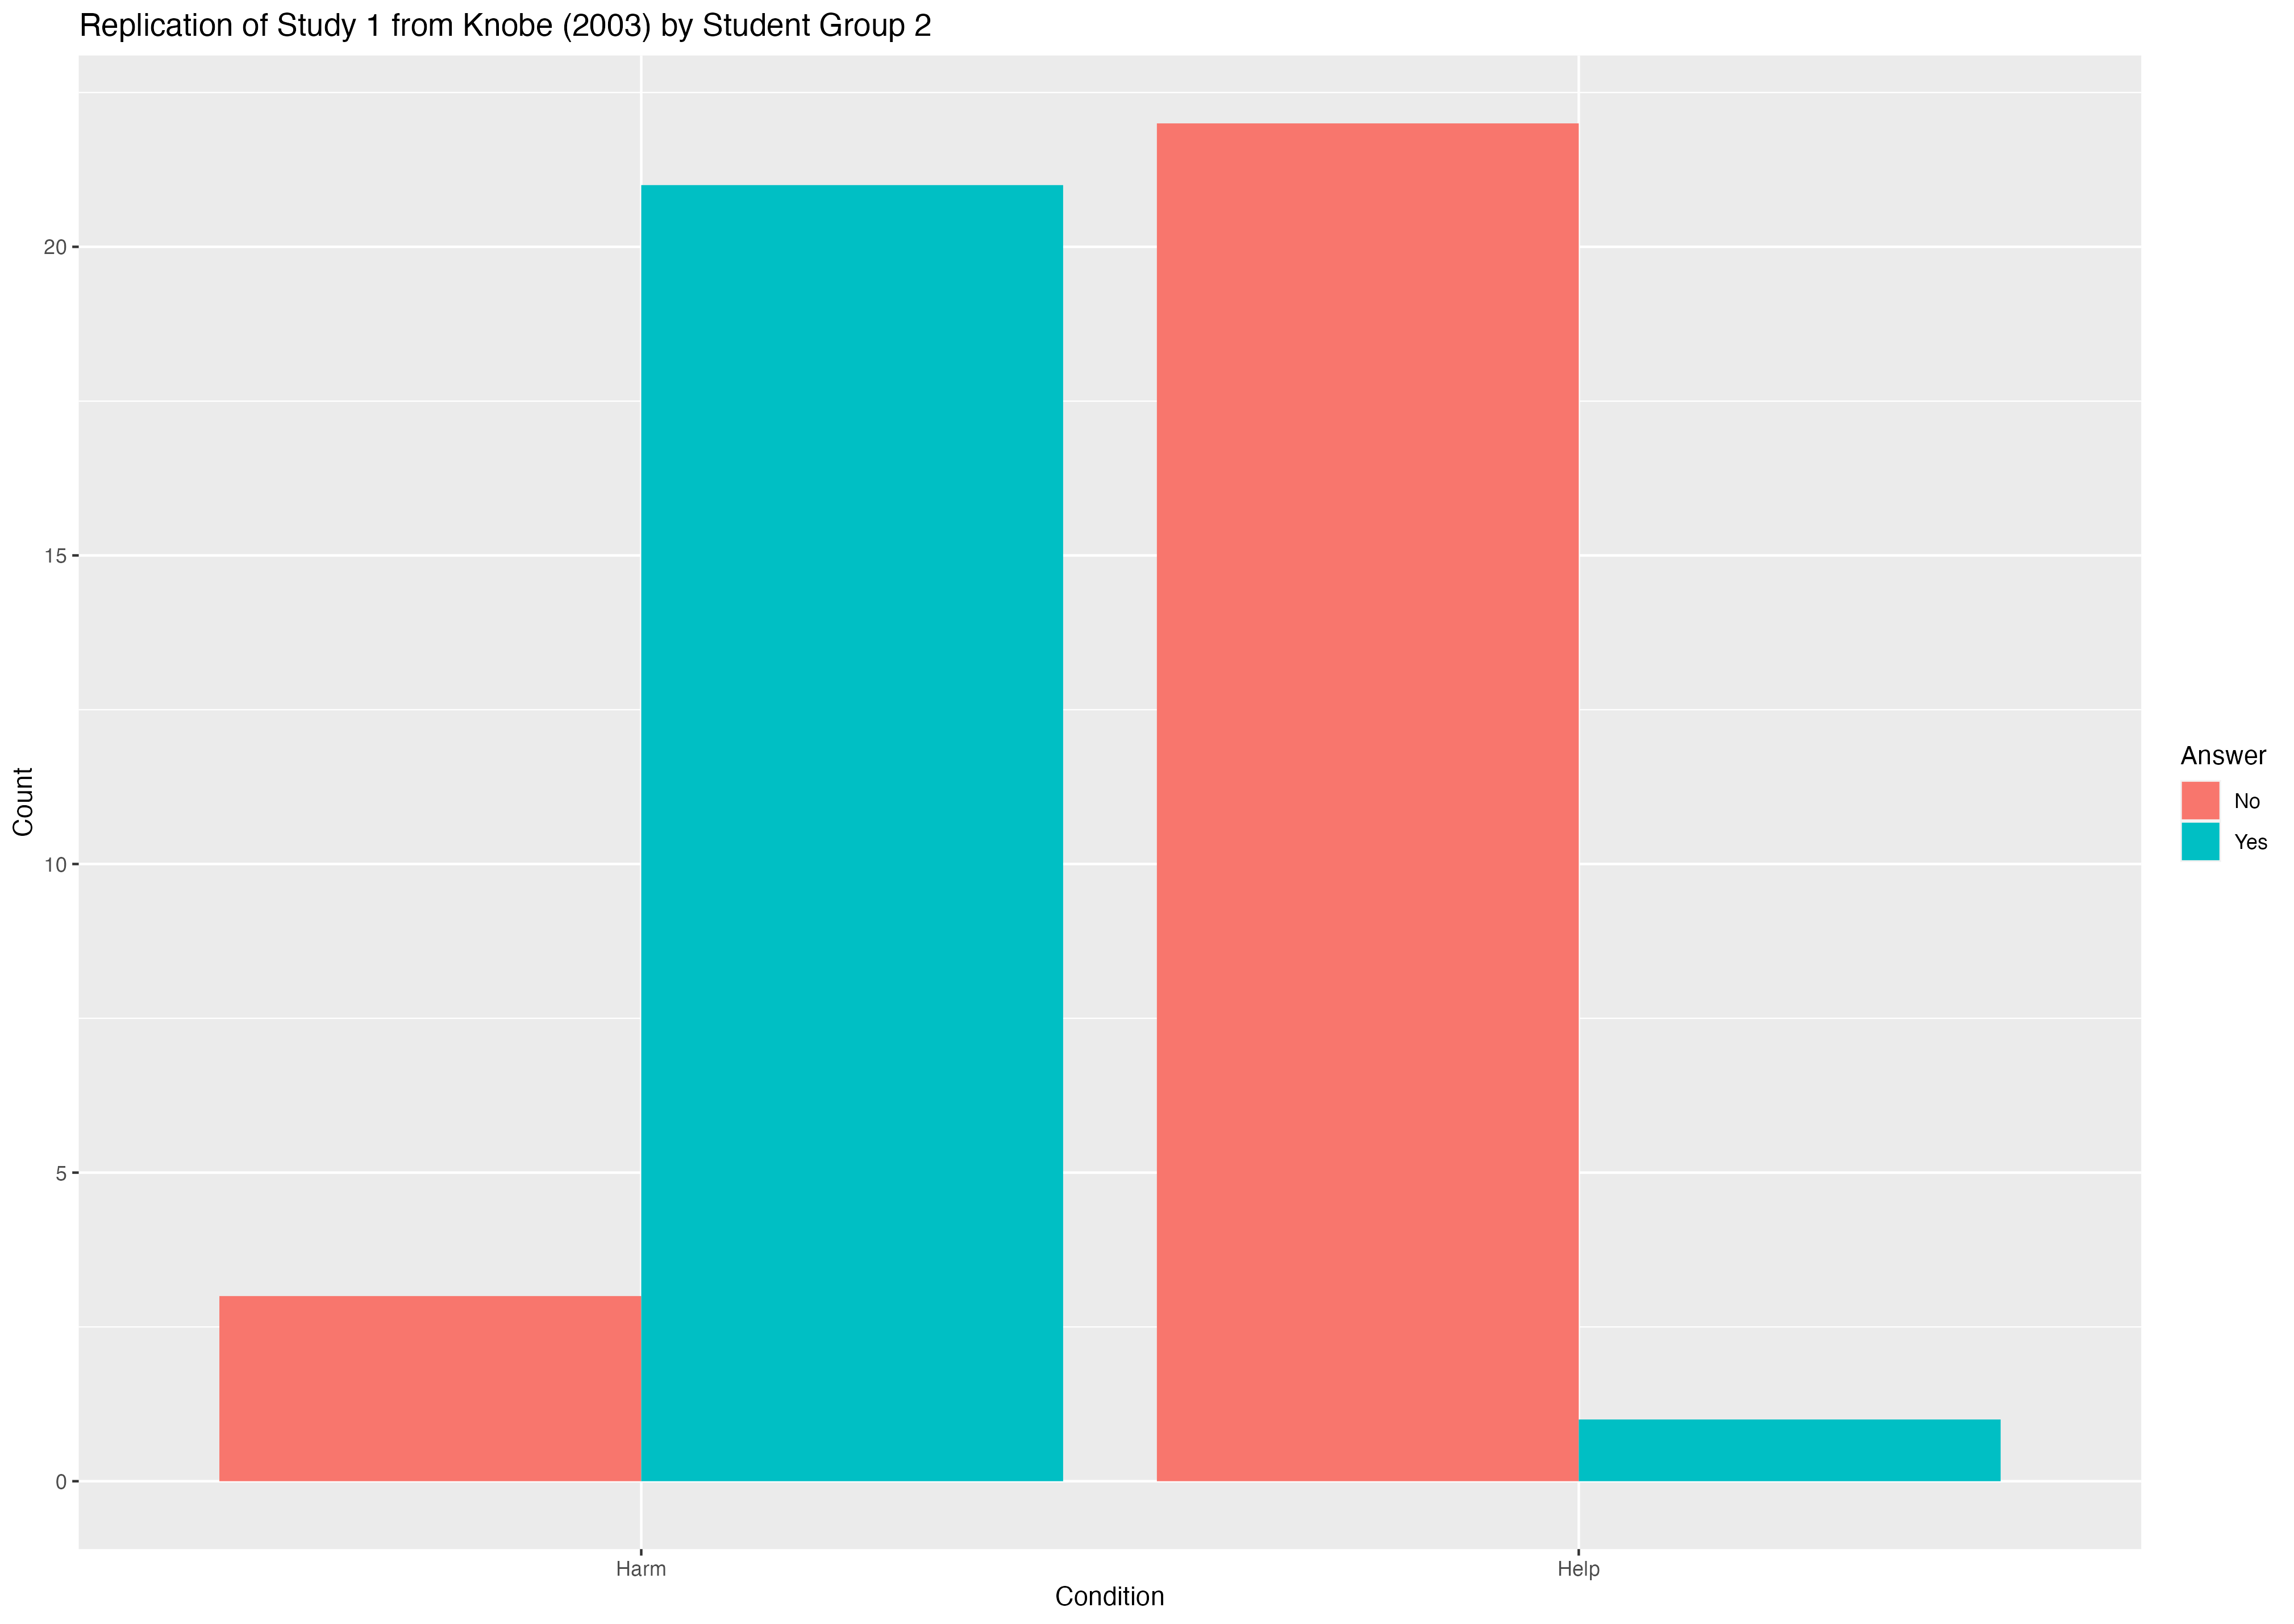
\includegraphics[width=0.75\linewidth]{figures/replication_knobe_fig_3.png}}\\
      \frame{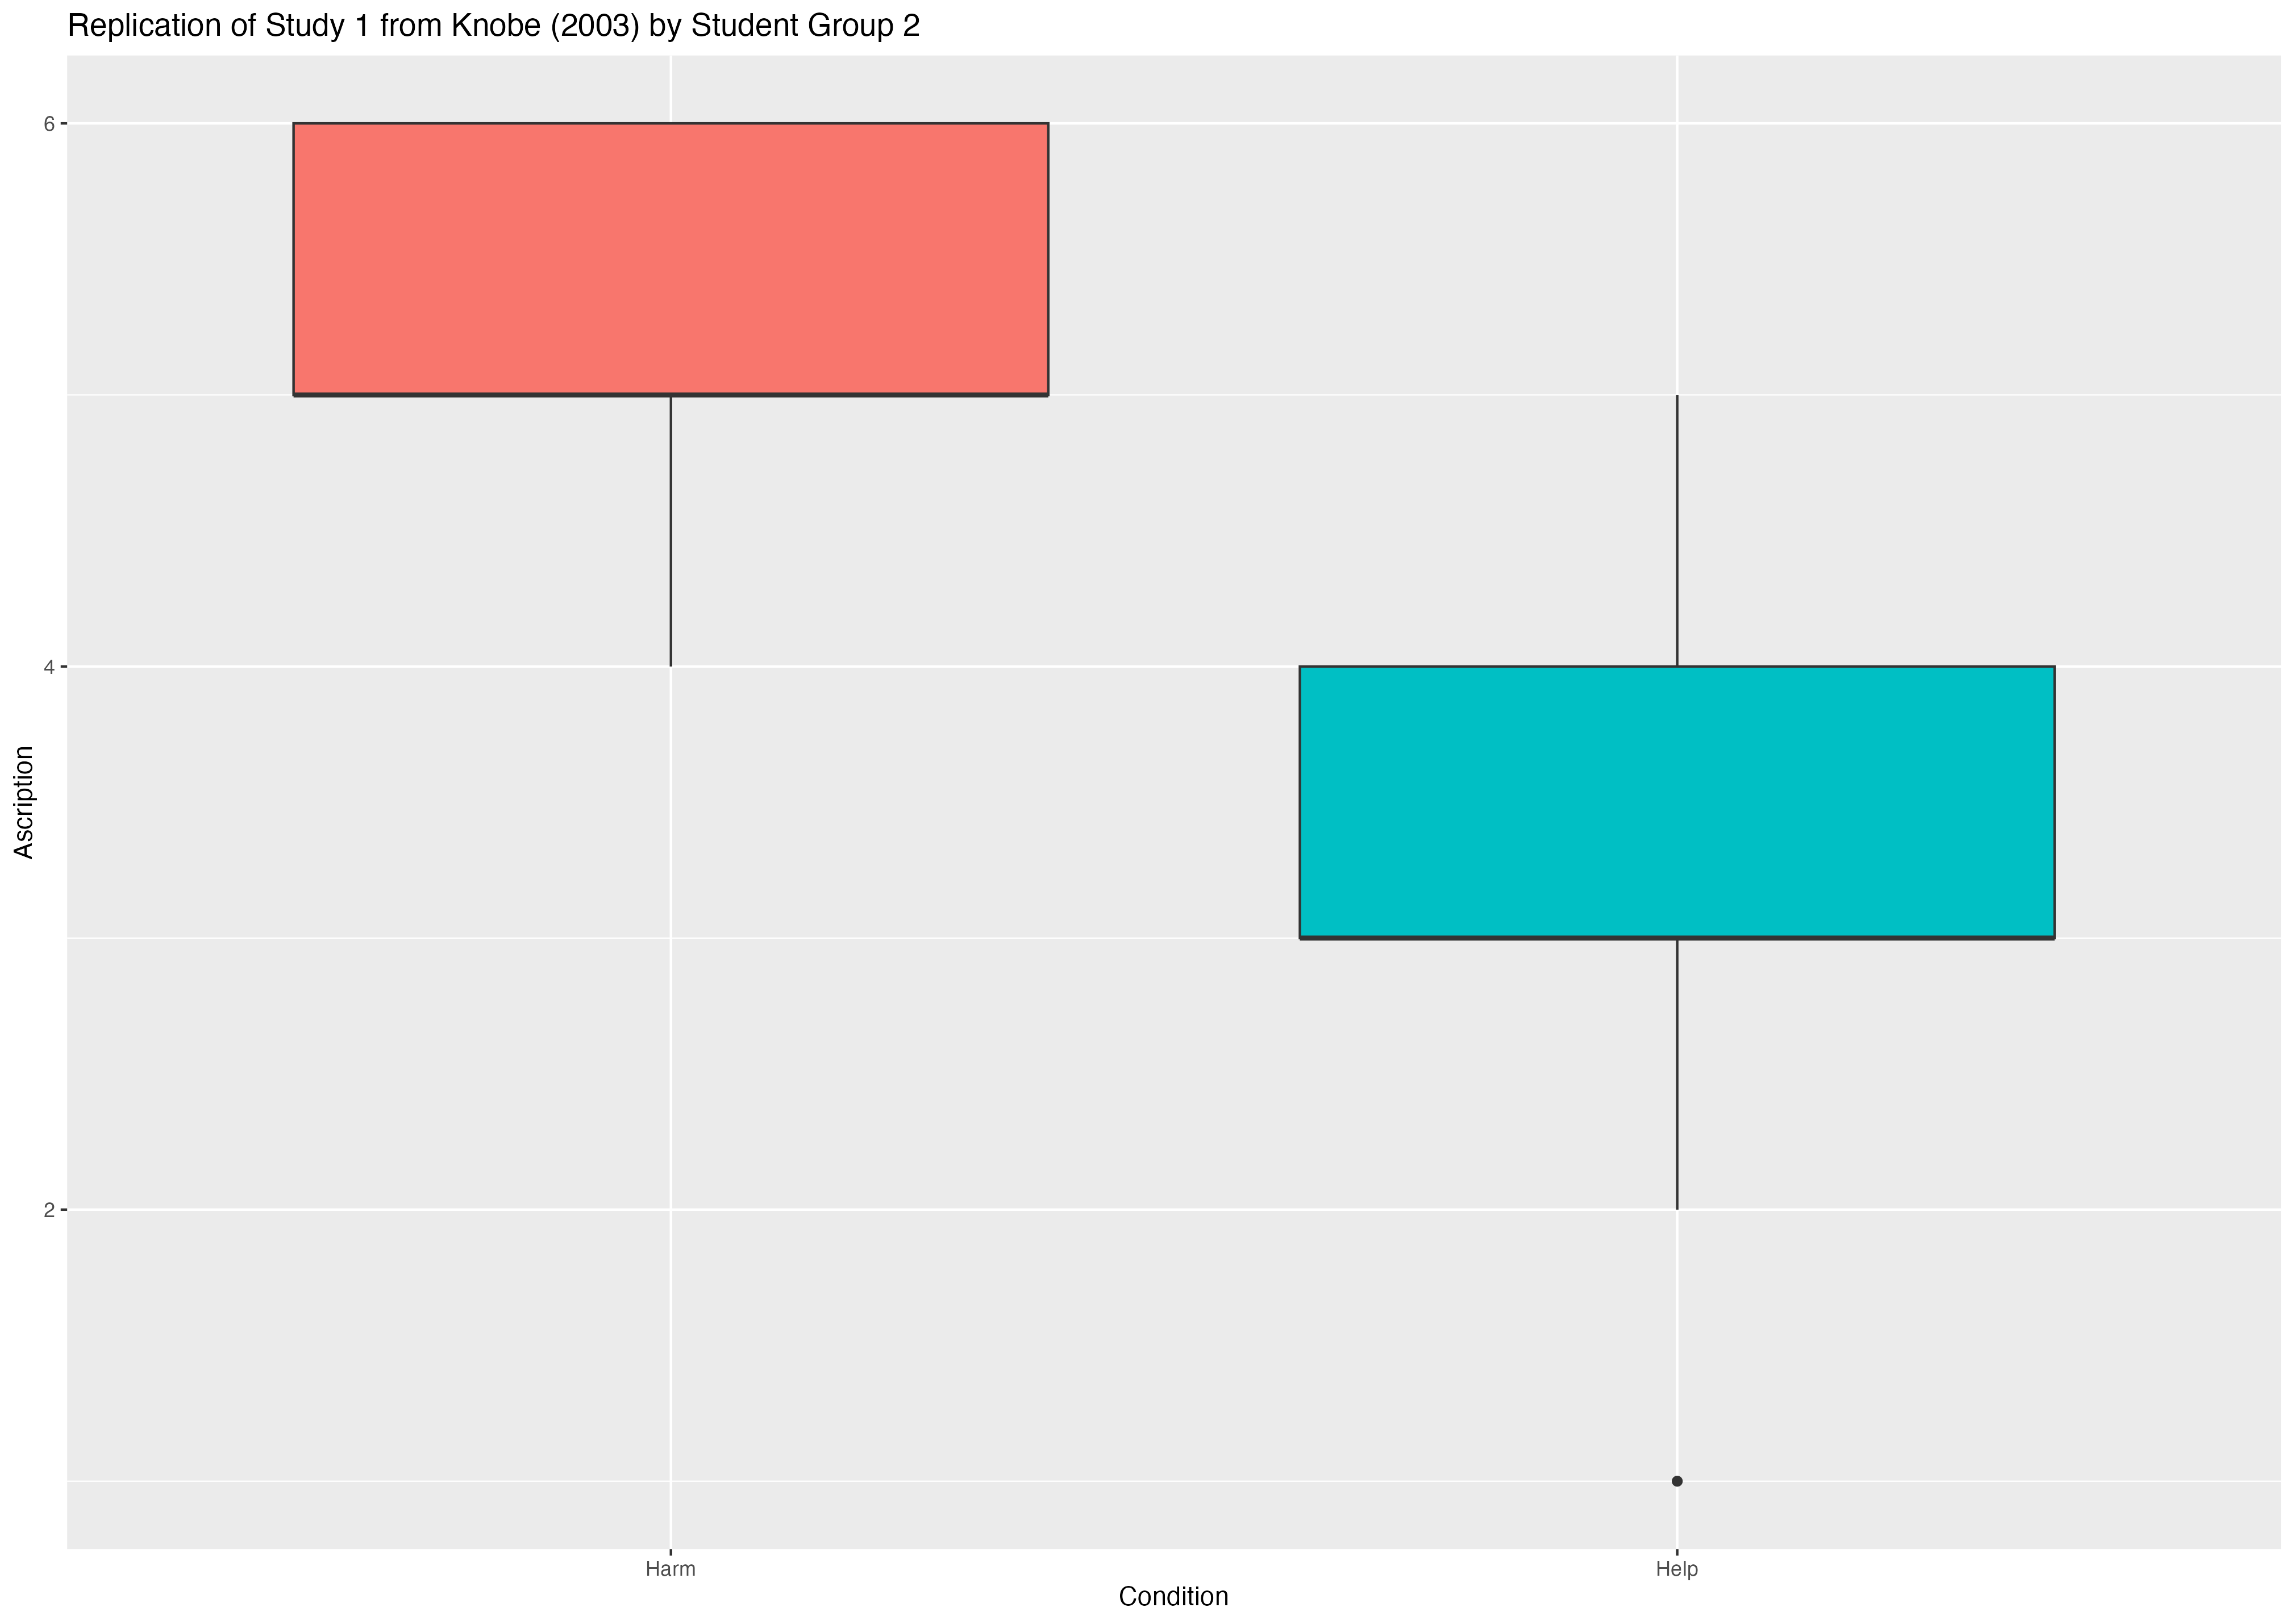
\includegraphics[width=0.75\linewidth]{figures/replication_knobe_fig_4.png}}\\
   \end{center}
\end{multicols}
\textbf{Antwort:} $\chi^2(df=1,n=47)=29,361$, $p<0,001$; $w=0,833$\\

\medskip
\textbf{Zuschreibung:} Schaden $M=5,21$, $SD=0,588$; Helfen $M=3,26$, $SD=0,915$; $t=8,64$, $p<0,001$; $d=2,53$
\end{frame}


%%%%%%%%%%%%
% FOLIE 38 %
%%%%%%%%%%%%
\begin{frame}{\vspace*{10mm}4\hspace*{1em}Ergebnisse der Replikationsstudie}
\textbf{Ergebnisse Gruppe 3}\\
\begin{multicols}{2}
   \begin{center}
      \frame{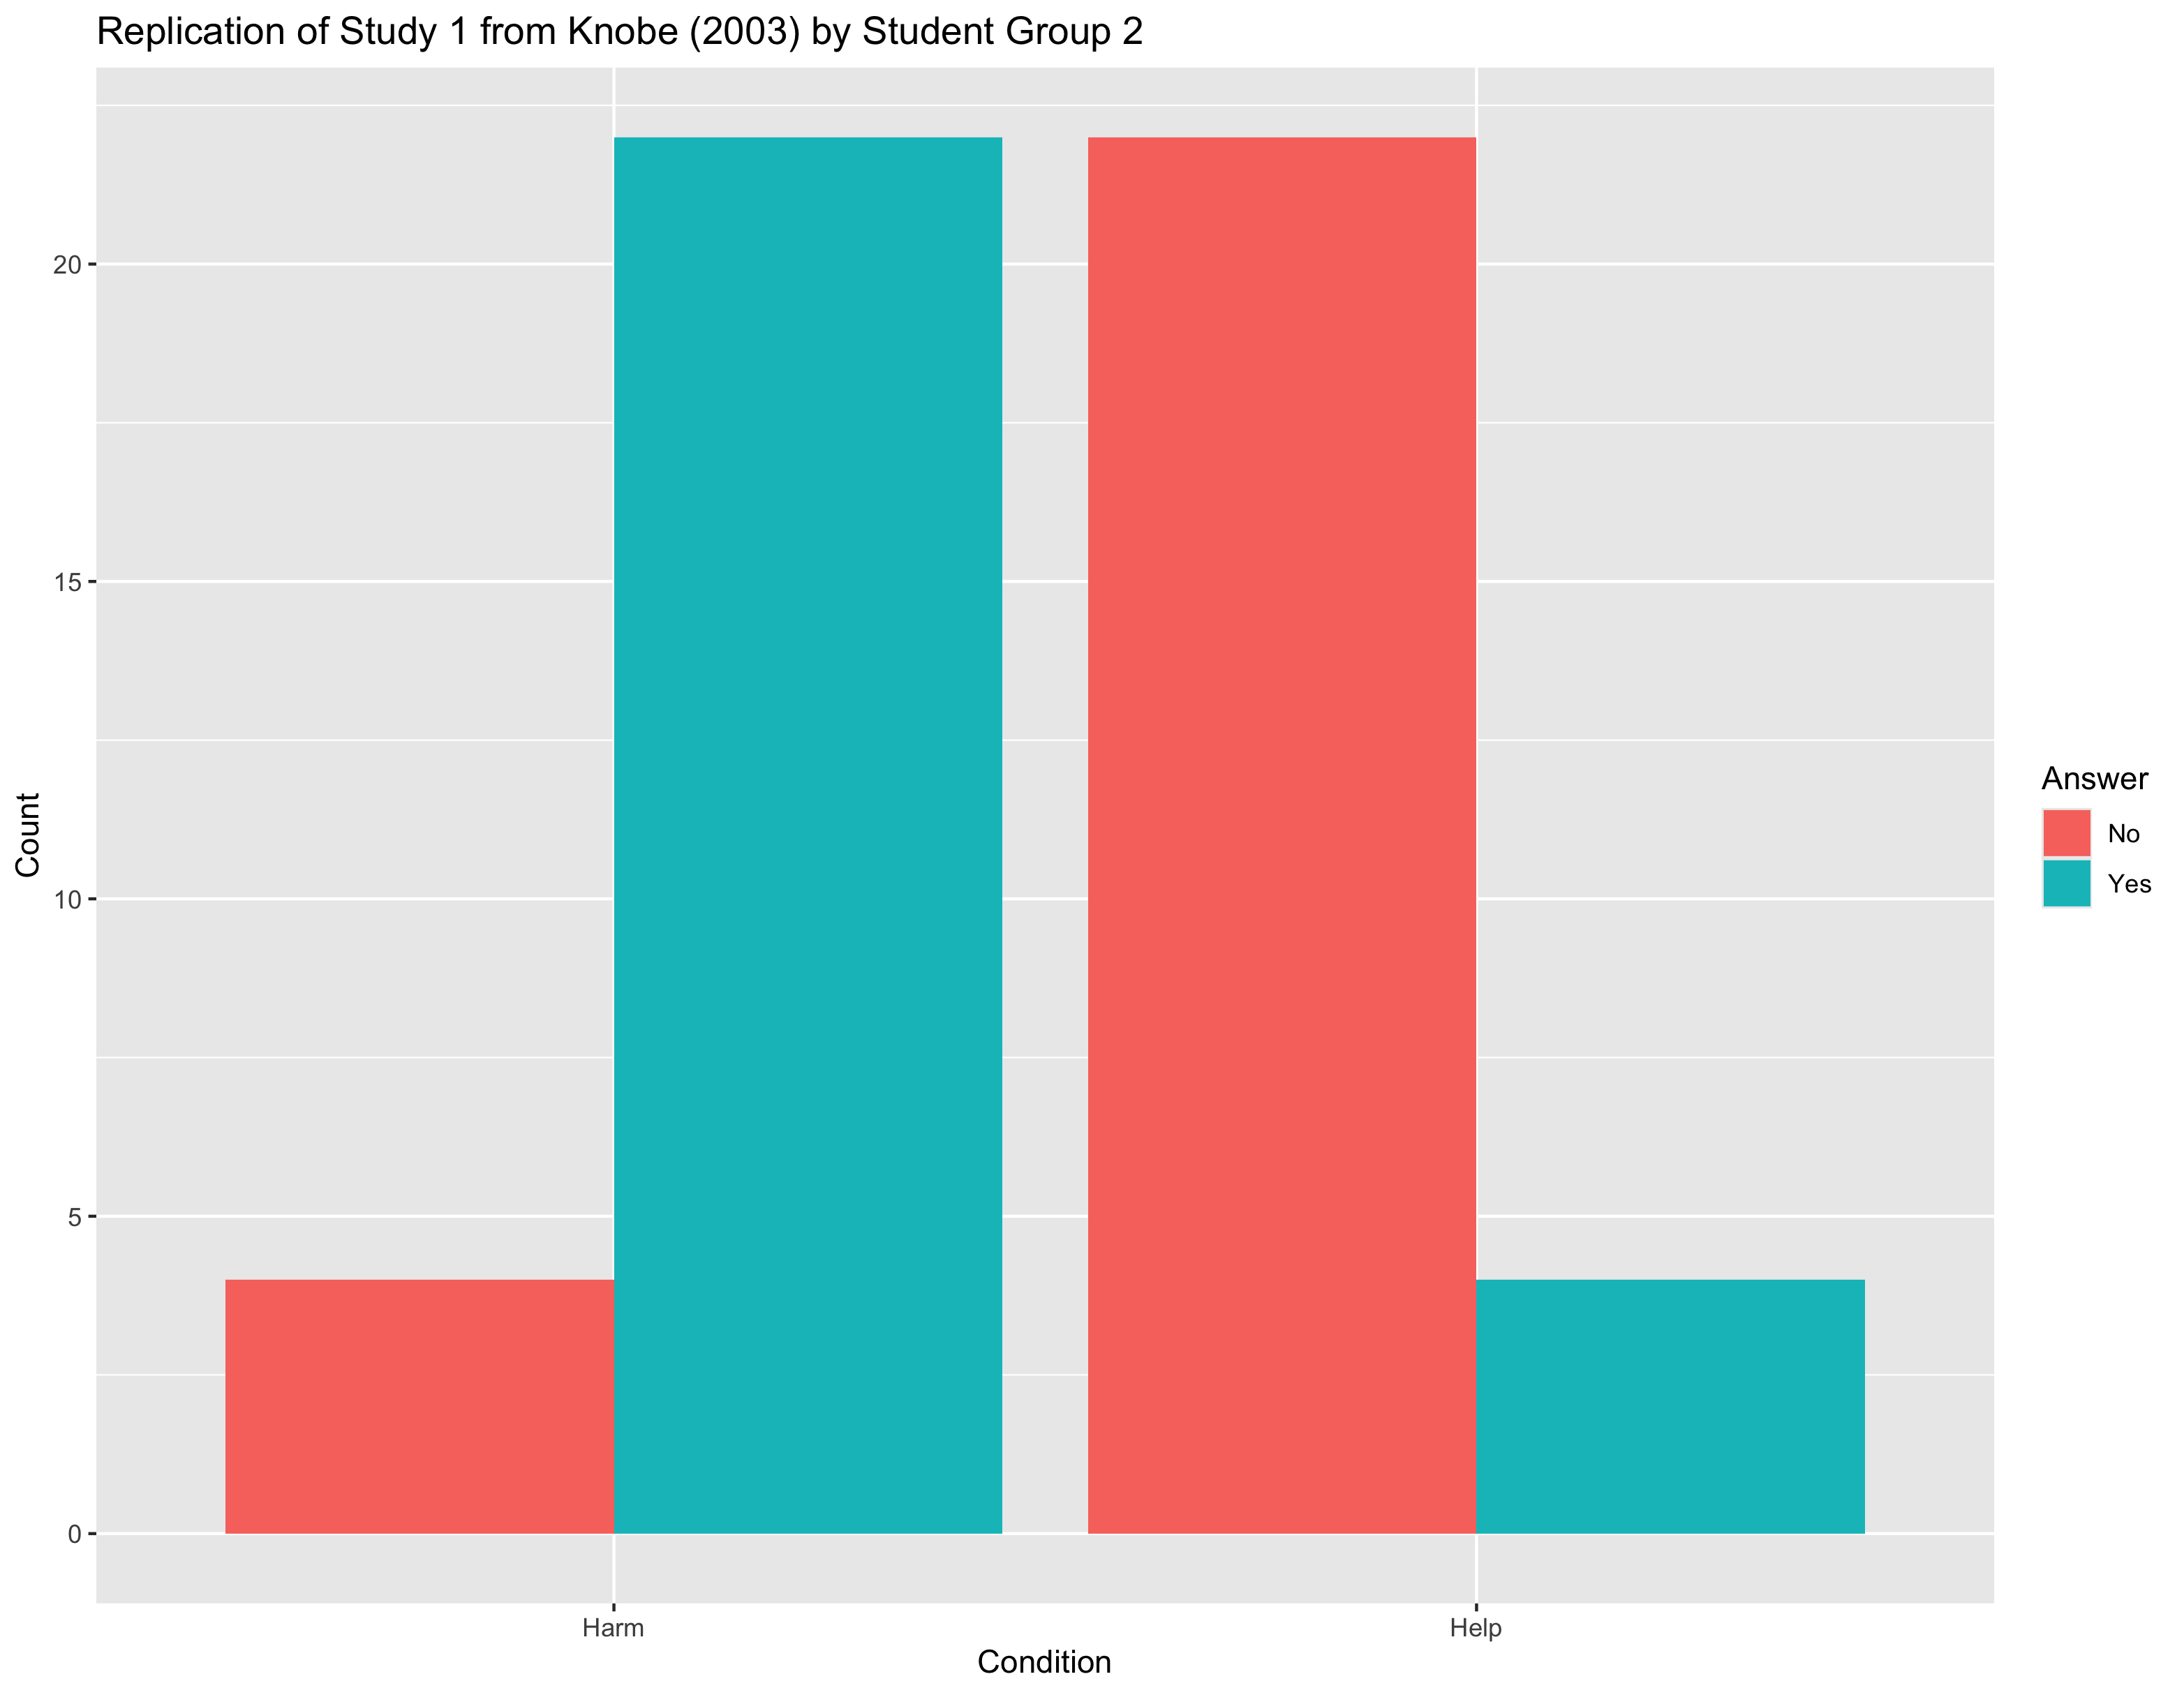
\includegraphics[width=0.75\linewidth]{figures/replication_knobe_fig_5.png}}\\
      \frame{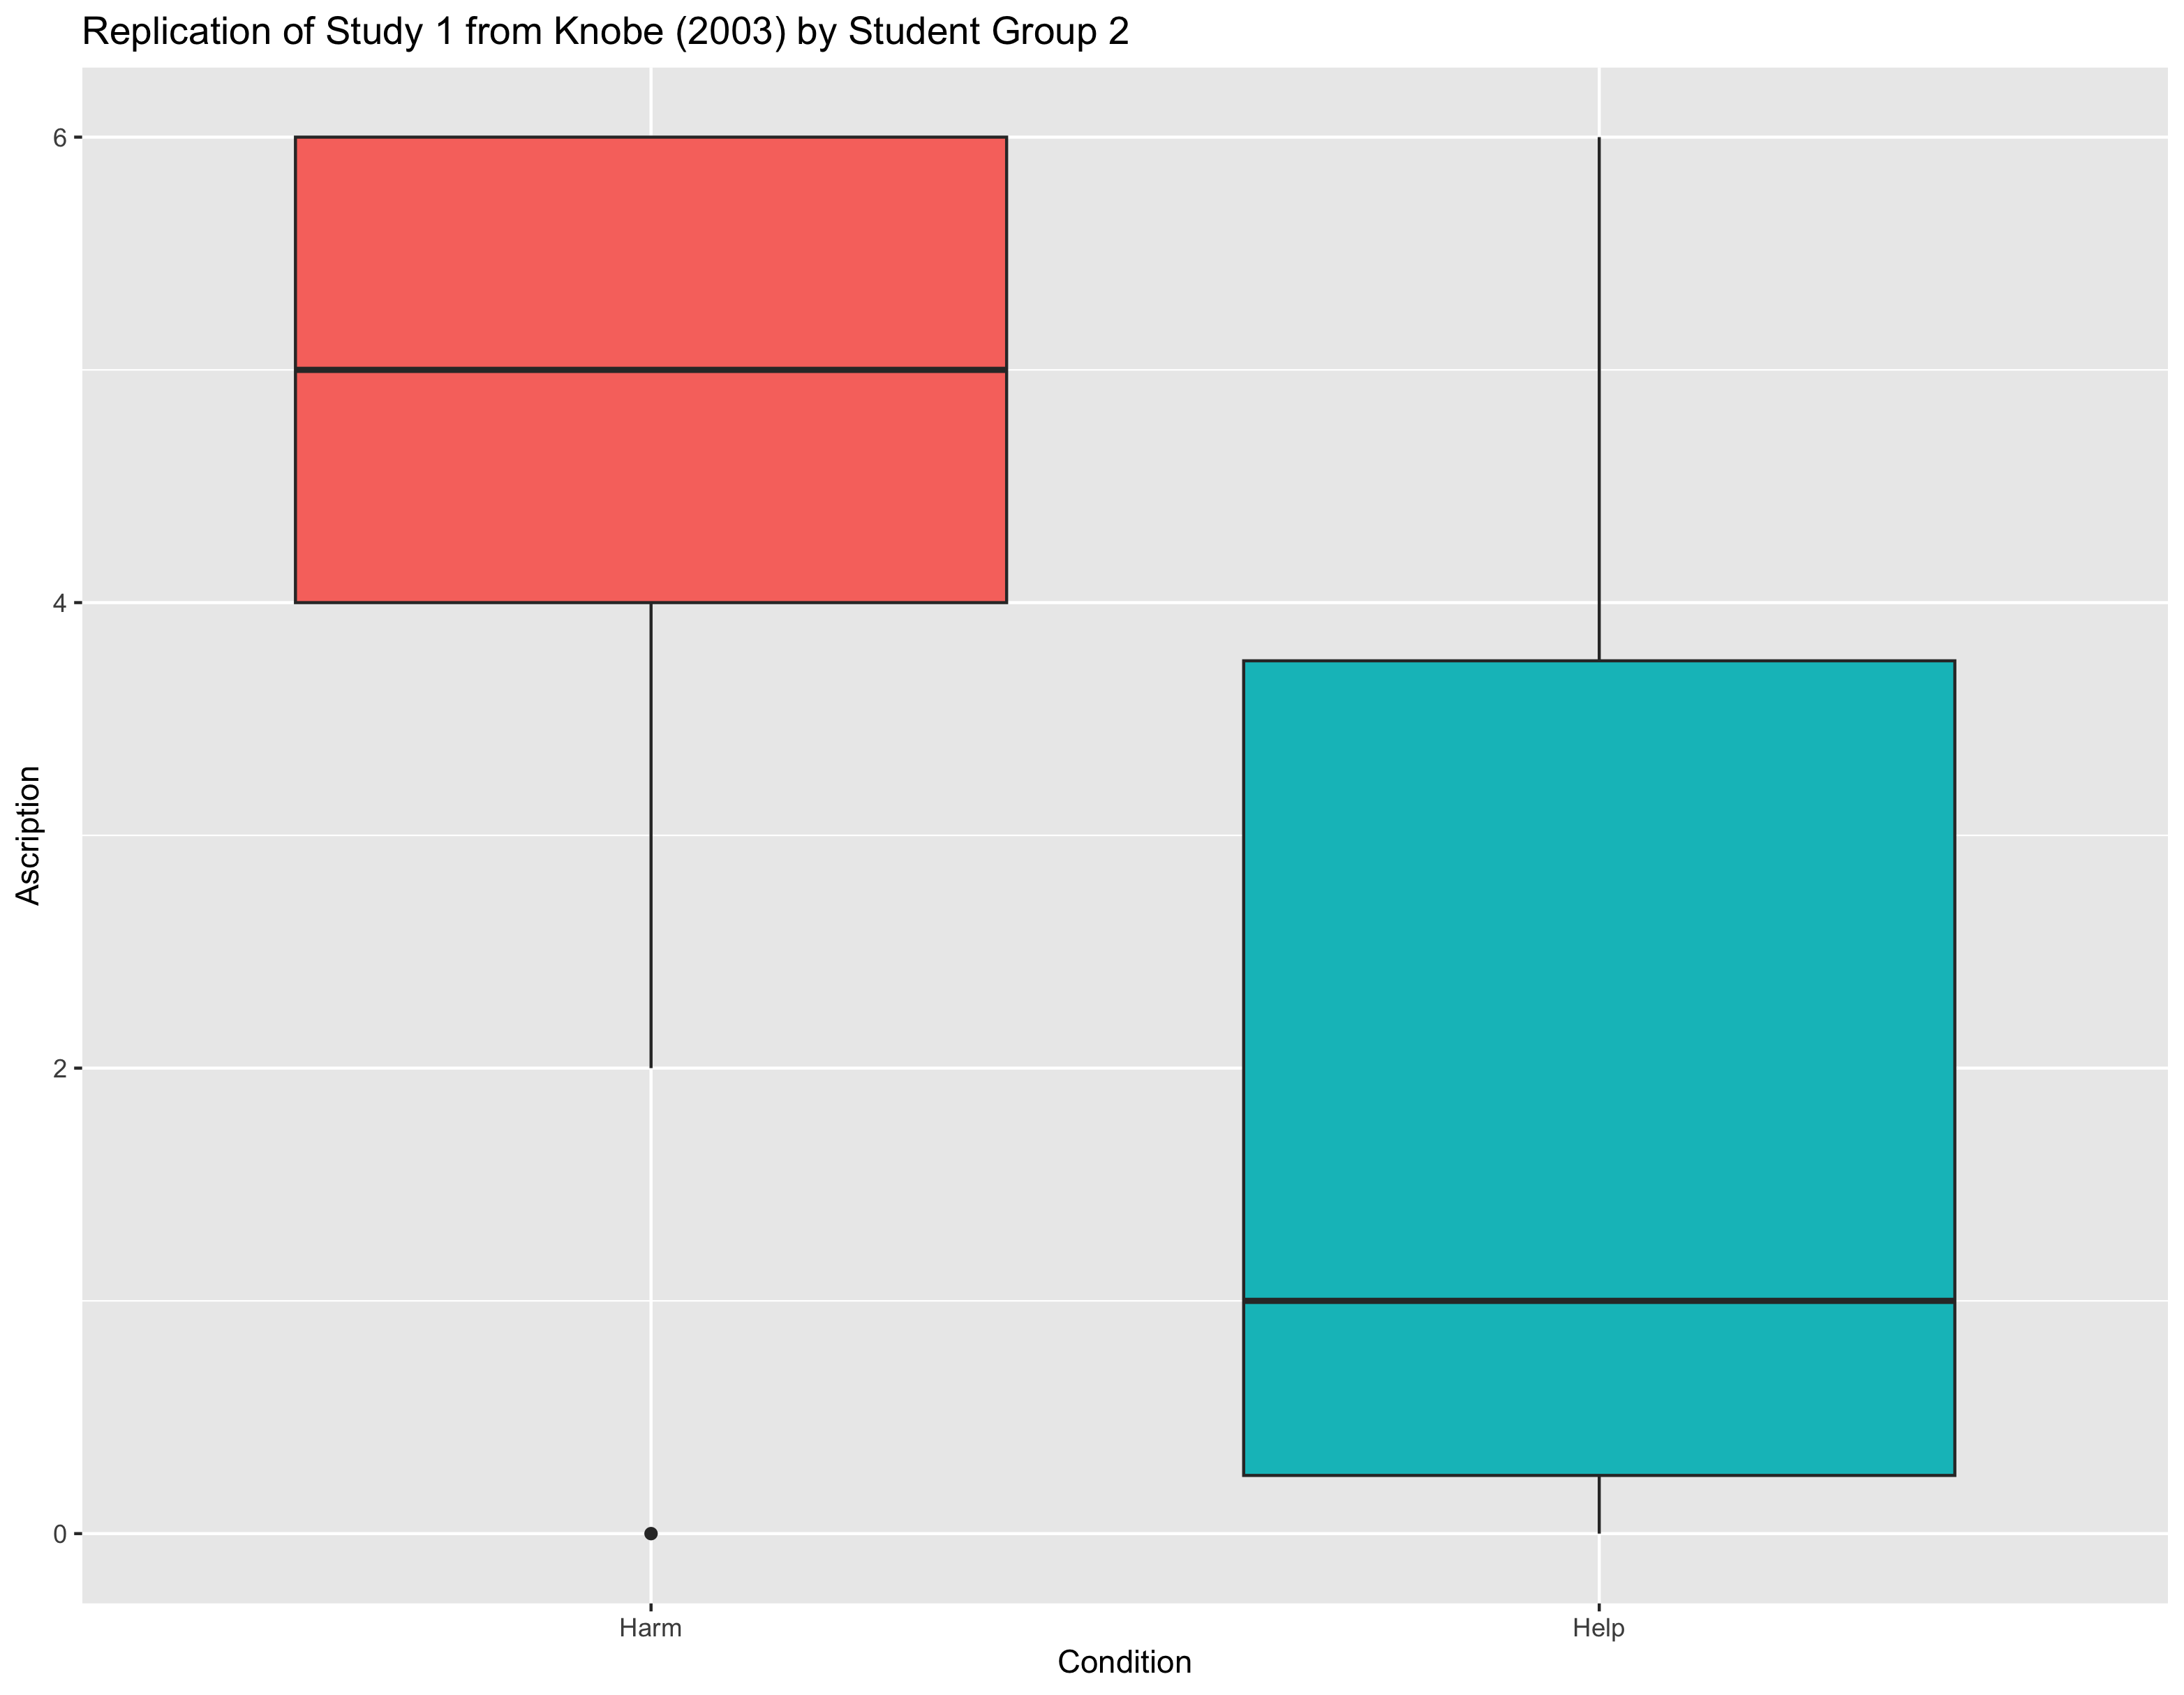
\includegraphics[width=0.75\linewidth]{figures/replication_knobe_fig_6.png}}\\
   \end{center}
\end{multicols}
\textbf{Antwort:} $\chi^2(df=1,n=52)=22,231$, $p<0,001$; $w=0,692$\\

\medskip
\textbf{Zuschreibung:} Schaden $M=4,77$, $SD=1,56$; Helfen $M=2,04$, $SD=1,93$; $t=5,62$, $p<0,001$; $d=1,56$
\end{frame}


%%%%%%%%%%%%%%%%%%%%%%%%%%%%%%%%%%
% FOLIE 39 – VORBEREITUNG THEMEN %
%%%%%%%%%%%%%%%%%%%%%%%%%%%%%%%%%%
\begin{frame}
\begin{overlayarea}{\textwidth}{0.81\paperheight}{
   \vspace*{11mm}
   \usebeamerfont{title}\textcolor{uolblue}
   {5\hspace*{1em}Vorbereitung der eigenen Themen}
}
\end{overlayarea}
\end{frame}


%%%%%%%%%%%%
% FOLIE 40 %
%%%%%%%%%%%%
\begin{frame}{\vspace*{10mm}5\hspace*{1em}Vorbereitung der eigenen Themen}
\textbf{Gruppenzuordnung}
   \begin{itemize}
      \item Gruppe 1 (Bavendiek, Laesecke, Wiechmann): \textbf{Ziviler Ungehorsam und Gewalt}
      \item Gruppe 2 (Kratzer, Lüttich, Rüterbories): \textbf{Autonome Systeme als moralische Akteure}
      \item Gruppe 3 (Göbbels, Gronotte, Hinkel, Schwarz): \textbf{Moralische Verpflichtung und Nähe}
   \end{itemize}
\end{frame}


%%%%%%%%%%%%
% FOLIE 41 %
%%%%%%%%%%%%
\begin{frame}{\vspace*{10mm}5\hspace*{1em}Vorbereitung der eigenen Themen}
\textbf{Recherche}\\
\smallskip
\url{https://philpapers.org/browse/experimental-philosophy}

\bigskip
\begin{center}
   \frame{
\includegraphics[width=0.55\linewidth]{figures/philpapers.png}}\\
\end{center}
\end{frame}


%%%%%%%%%%%%%%%%%%%%%%%%%%%%%
% FOLIE 42 – ANALYSE THEMEN %
%%%%%%%%%%%%%%%%%%%%%%%%%%%%%
\begin{frame}
\begin{overlayarea}{\textwidth}{0.81\paperheight}{
   \vspace*{11mm}
   \usebeamerfont{title}\textcolor{uolblue}
   {6\hspace*{1em}Analyse der eigenen Themen}
}
\end{overlayarea}
\end{frame}


%%%%%%%%%%%%
% FOLIE 43 %
%%%%%%%%%%%%
\begin{frame}{\vspace*{10mm}6\hspace*{1em}Analyse der eigenen Themen}
\textbf{Gruppe 1: Ziviler Ungehorsam und Gewalt}\\
\begin{center}
   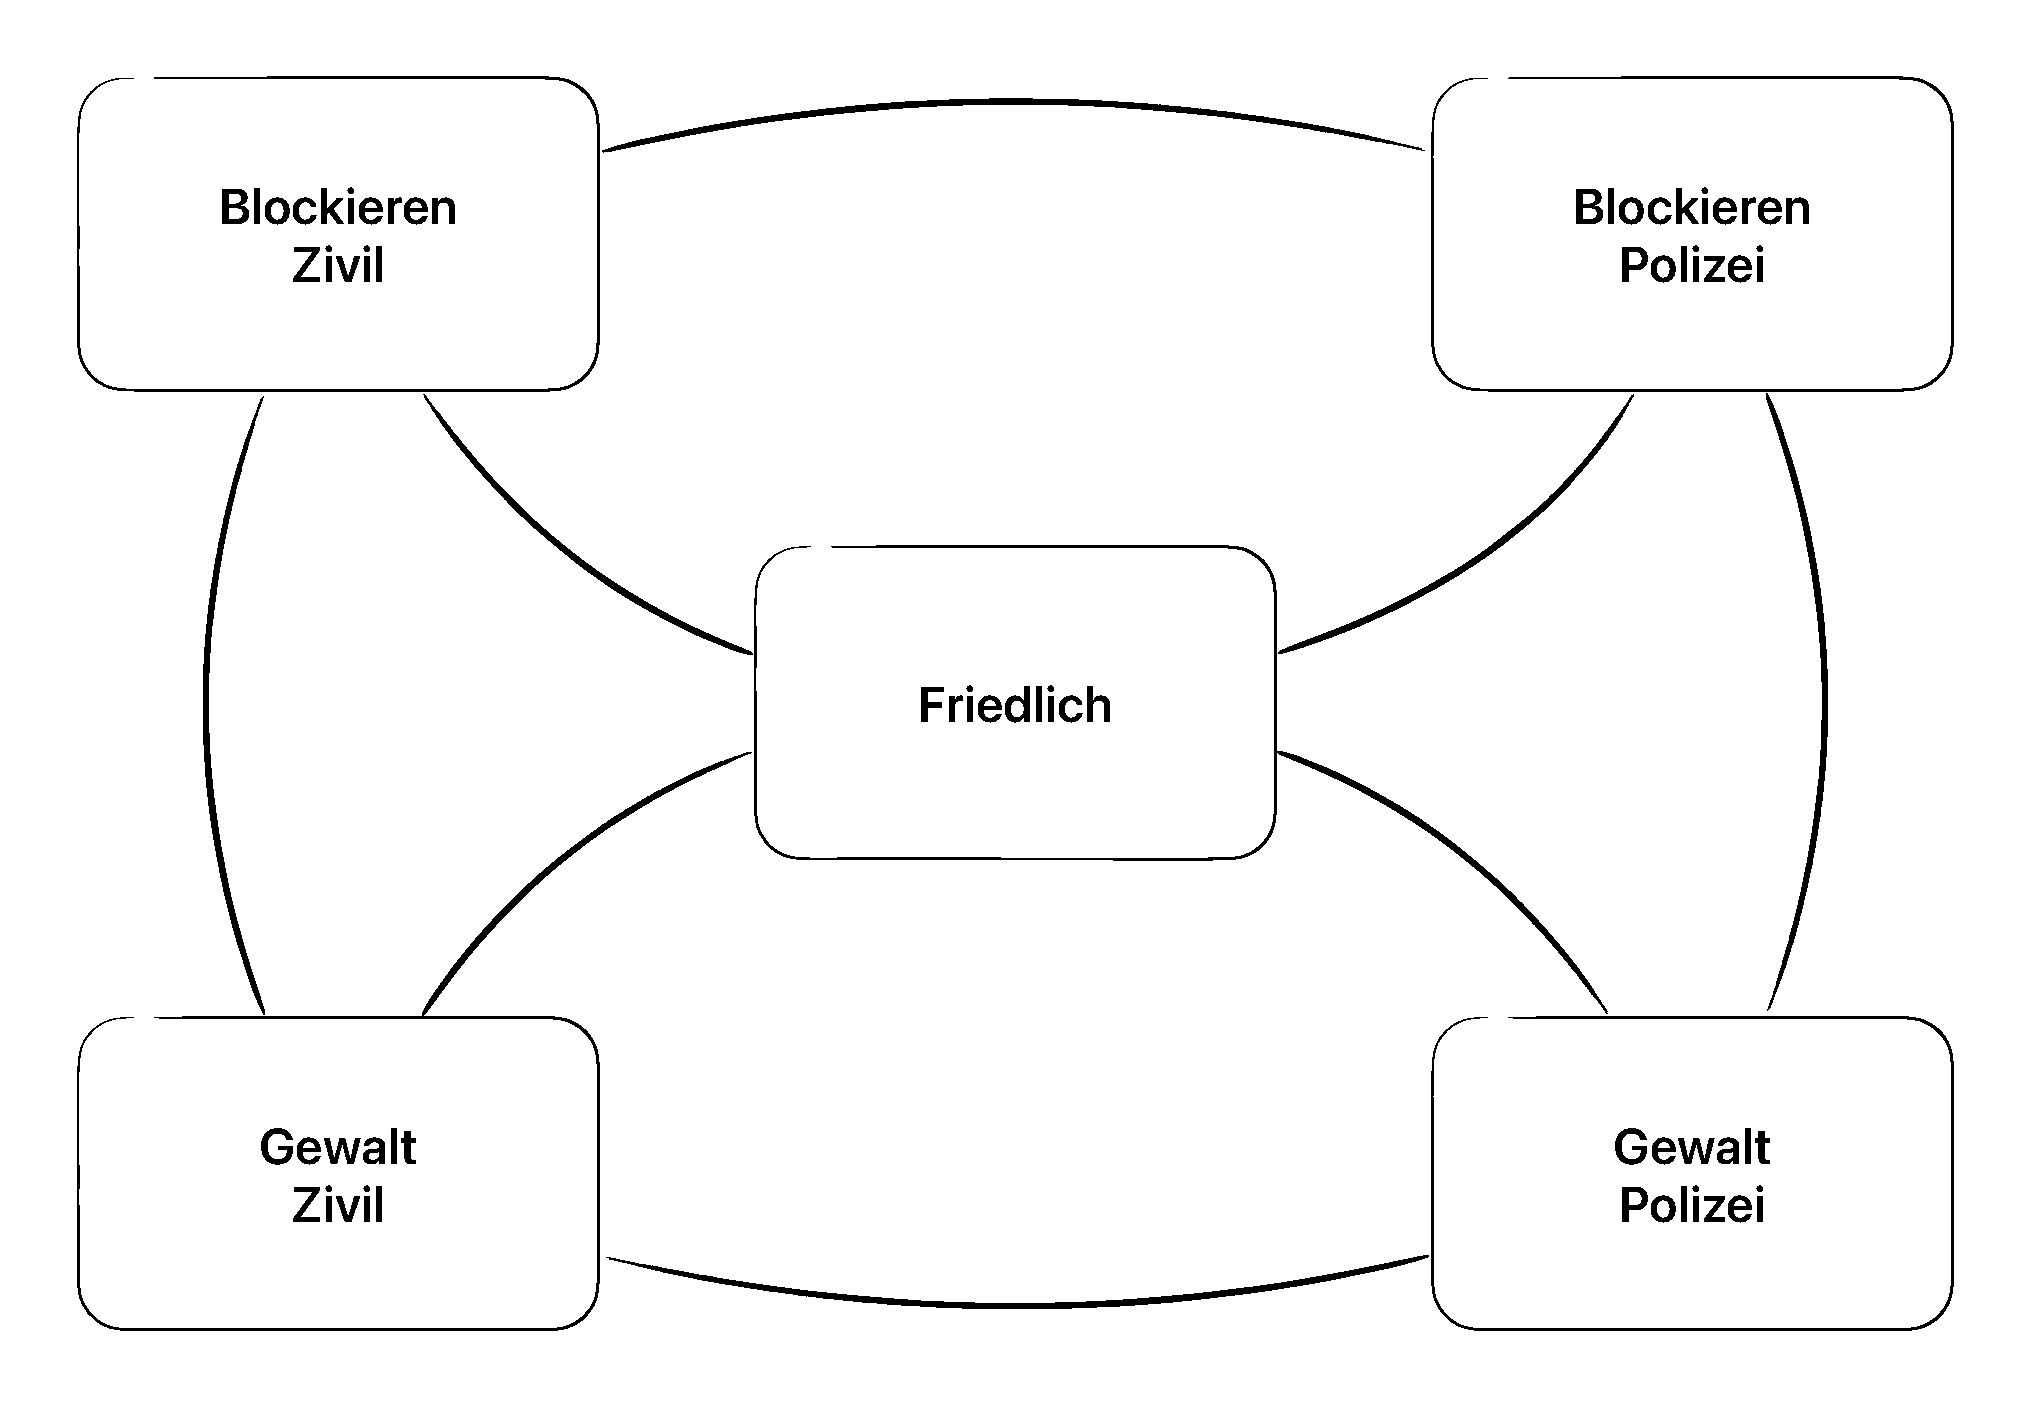
\includegraphics[width=0.5\linewidth]{figures/civil_disobedience_structure.pdf}\\
\end{center}
\end{frame}


%%%%%%%%%%%%
% FOLIE 44 %
%%%%%%%%%%%%
\begin{frame}{\vspace*{10mm}6\hspace*{1em}Analyse der eigenen Themen}
\textbf{Gruppe 2: Autonome Systeme als moralische Akteure}\\
\begin{center}
   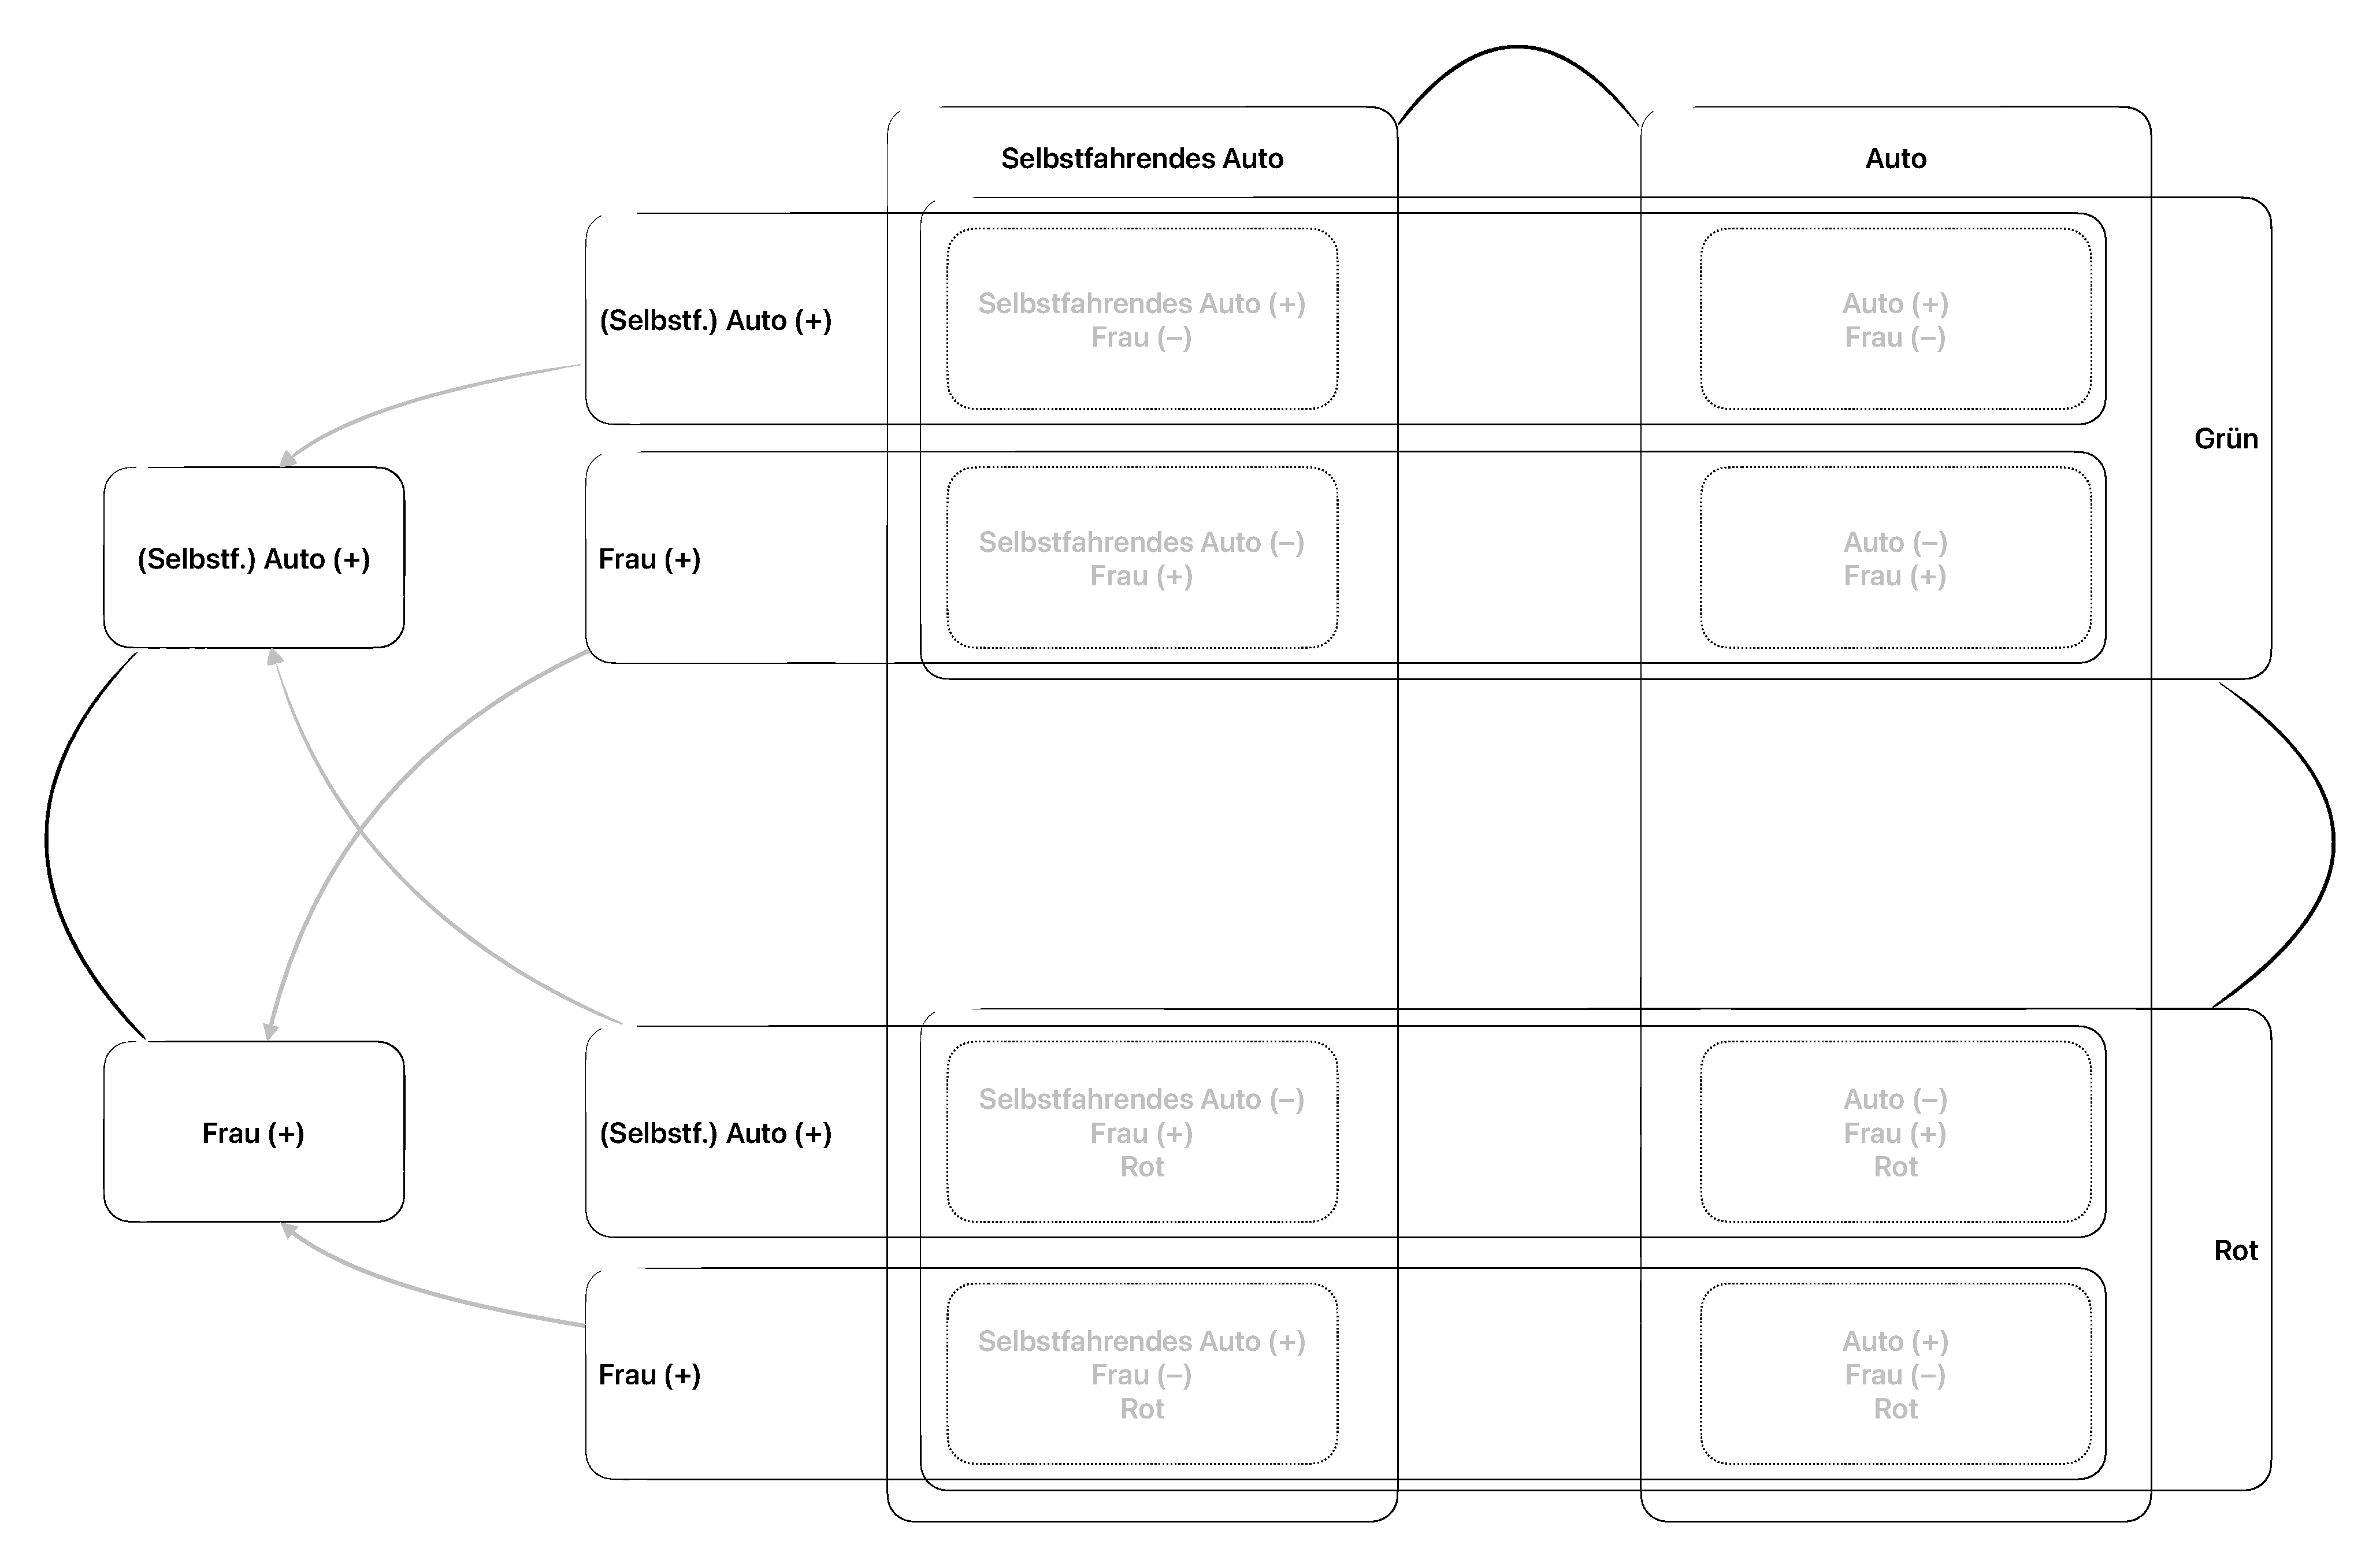
\includegraphics[width=0.5\linewidth]{figures/autonomous_systems_structure.pdf}\\
\end{center}
\end{frame}


%%%%%%%%%%%%
% FOLIE 45 %
%%%%%%%%%%%%
\begin{frame}{\vspace*{10mm}6\hspace*{1em}Analyse der eigenen Themen}
\textbf{Gruppe 3: Moralische Verpflichtung und Nähe}\\
\begin{center}
   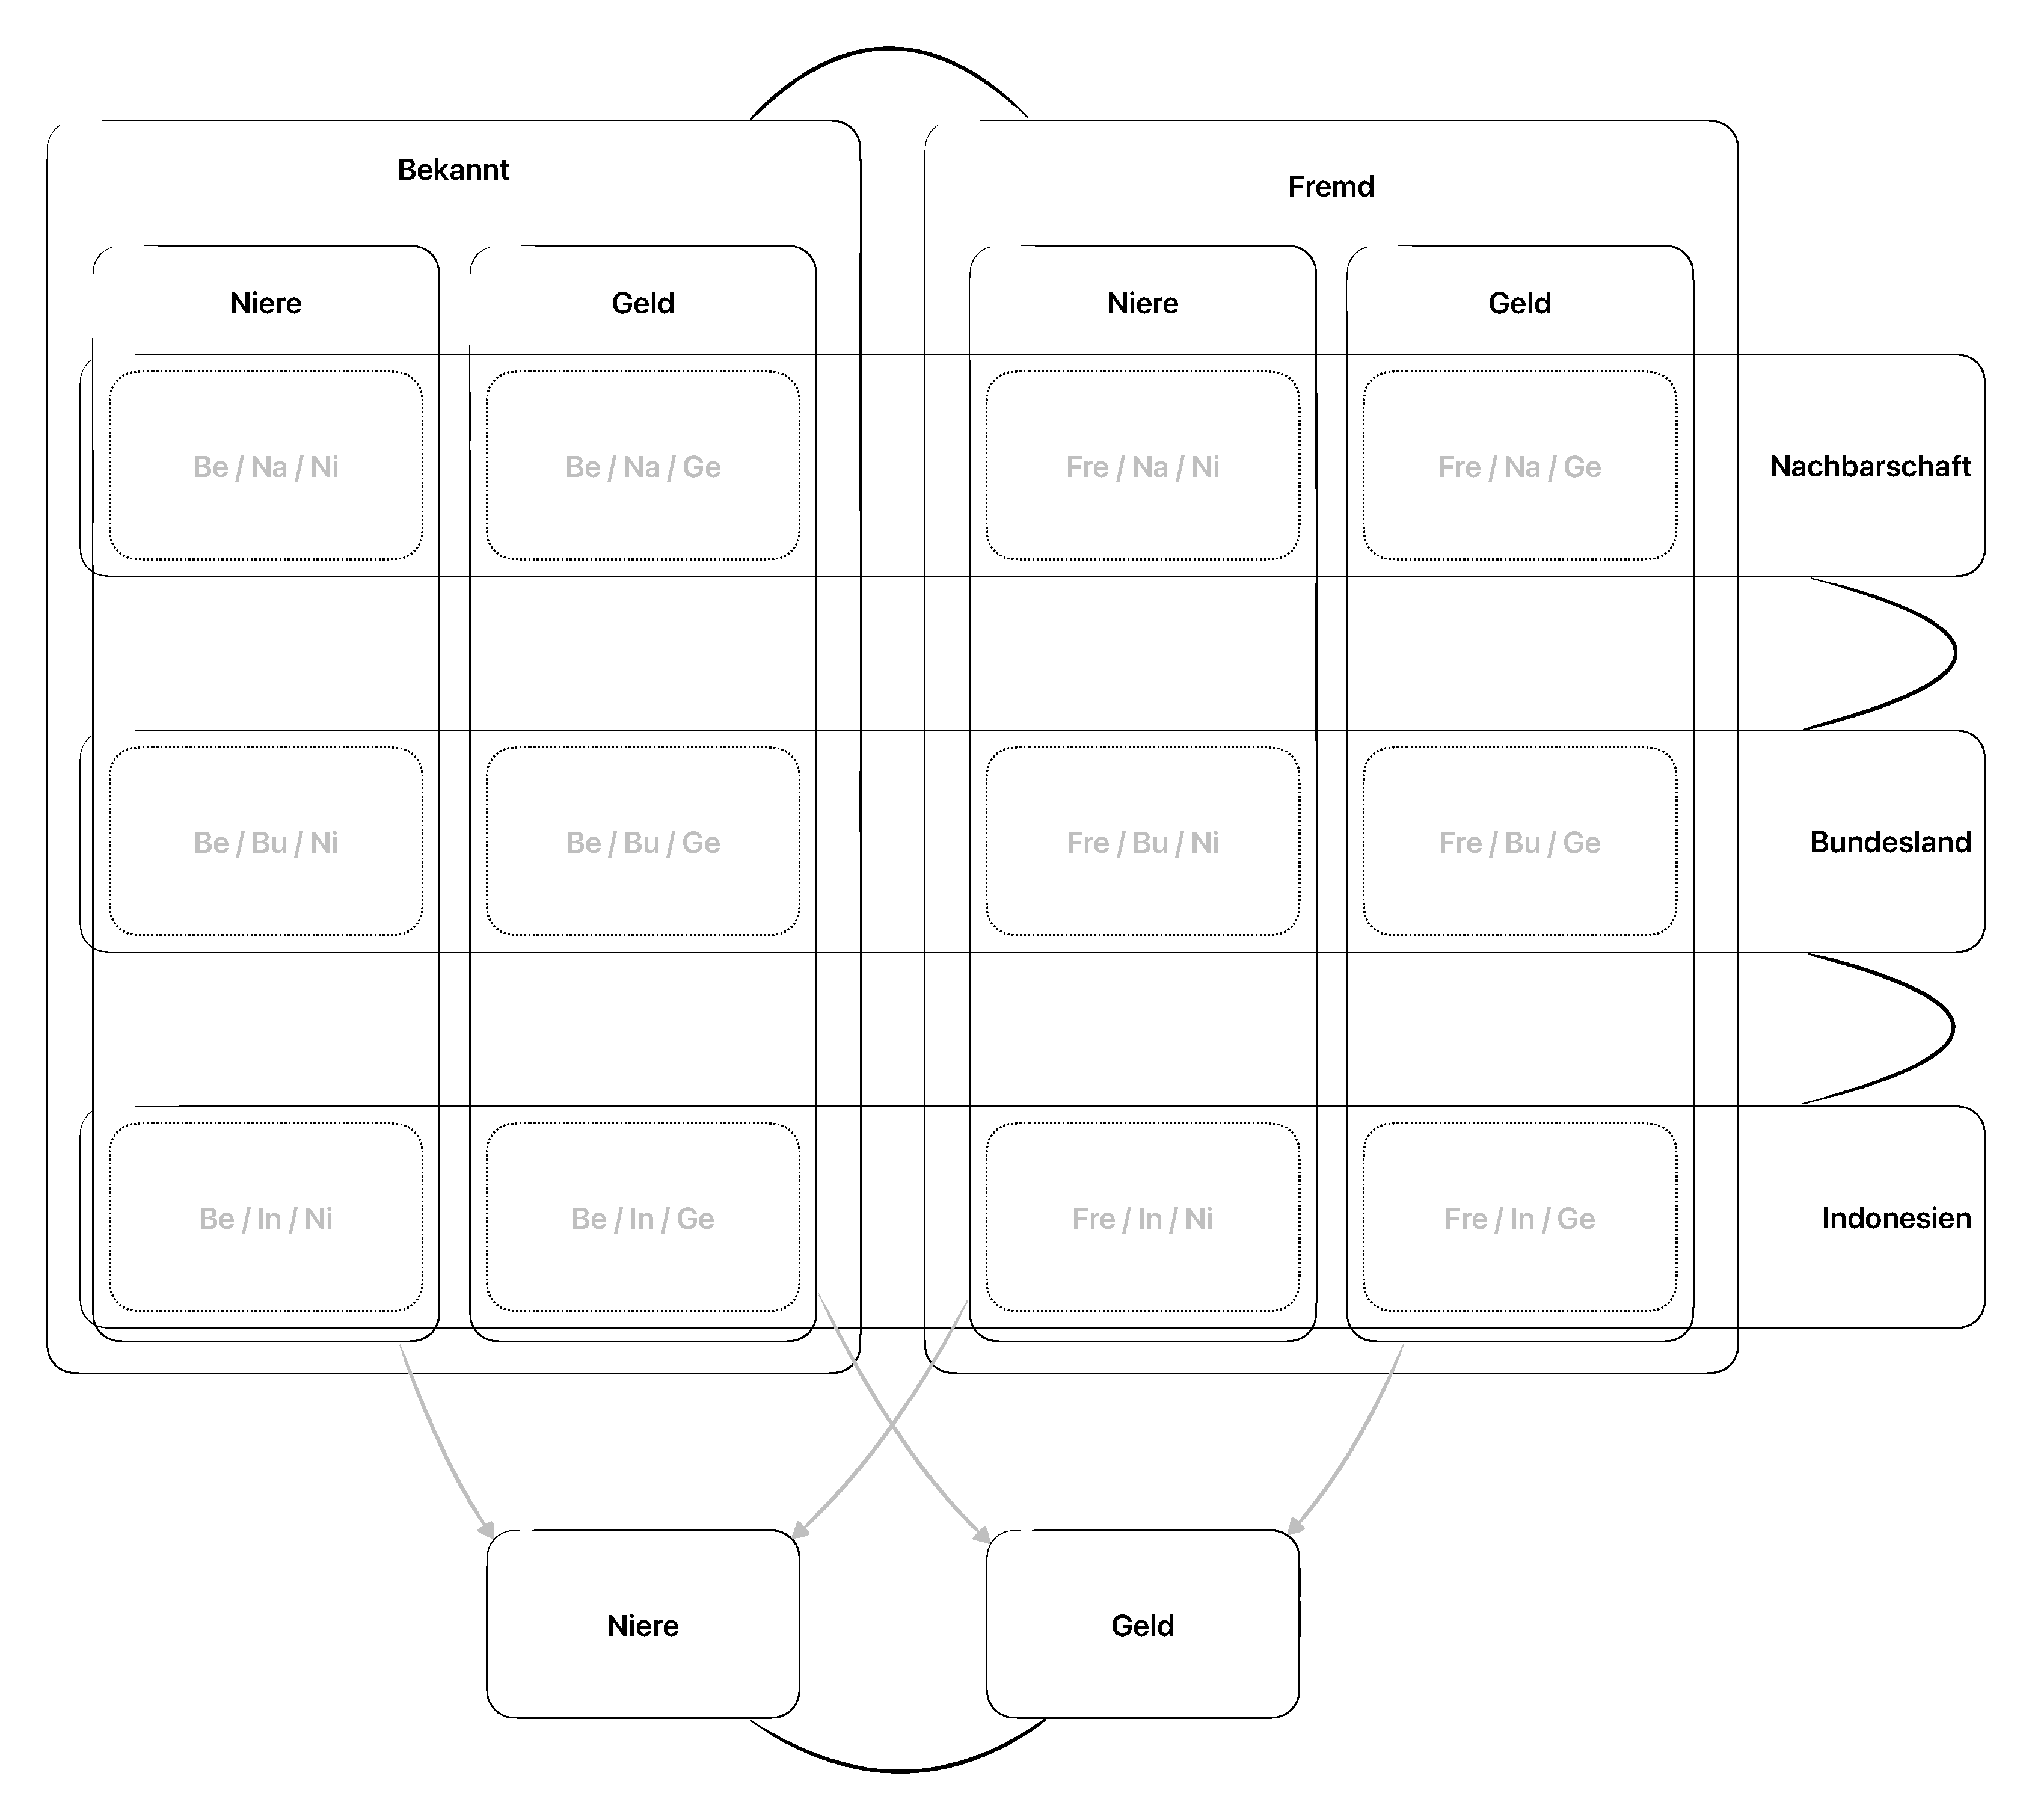
\includegraphics[width=0.5\linewidth]{figures/moral_obligation_structure.pdf}\\
\end{center}
\end{frame}


%%%%%%%%%%%%%%%%%%%%%%%%%%%
% FOLIE 46 – BIBLIOGRAFIE %
%%%%%%%%%%%%%%%%%%%%%%%%%%%
\begin{frame}{\vspace*{10mm}Bibliografie}
\vspace*{-5mm}
{\footnotesize
\begin{itemize}[label=,leftmargin=2em,itemindent=-2em]
   \item Bauer, Alexander Max, Stephan Kornmesser und Henrike Meyer (i.\,V.): \enquote{Constative and Performative Utterances, $\chi^2$ Tests, and LimeSurvey}. In: Stephan Kornmesser, Alexander Max Bauer, Mark Alfano, Aurélien Allard, Lucien Baumgartner, Florian Cova, Paul Engelhardt, Eugen Fischer, Henrike Meyer, Kevin Reuter, Justin Sytsma, Kyle Thompson und Marc Wyszynski: \textit{Experimental Philosophy for Beginners. A Gentle Introduction to Methods and Tools}. Cham: Springer. S.~19--88.
   \item Boslaugh, Sarah (2012): \textit{Statistics in a Nutshell. A Desktop Quick Reference}. 2.~Auflage. Sebastopol: O'Reilly.
   \item DATAtab Team (2024): \enquote{DATAtab. Online Statistics Calculator}, \url{https://datatab.net} (abgerufen am 17.04.2024).
   \item Gettier, Edmund (1963): \enquote{Is Justified True Belief Knowledge?}, \textit{Analysis} 23 (6), S.~121--123.
   \item Knobe, Joshua (2003): \enquote{Intentional Action and Side Effects in Ordinary Language}, \textit{Analysis} 63 (3), S.~190--194.
   \item Knobe, Joshua (2014): \enquote{Absichtliches Handeln und Nebeneffekte in der Alltagssprache}. Übers. von. Jürgen Schröder. In: Thomas Grundmann, Joachim Horvath und Jens Kipper (Hrsg.): \textit{Die Experimentelle Philosophie in der Diskussion}. Berlin: Suhrkamp. S.~96--101.
   \item Kuckartz, Udo, Stefan Rädiker, Thomas Ebert und Julia Schehl (2013): \textit{Statistik. Eine verständliche Einführung}. 2.~Auflage. Wiesbaden: Springer VS.
   \item Weinberg, Jonathan, Shaun Nichols und Stephen Stich (2001): \enquote{Normativity and Epistemic Intuitions}, \textit{Philosophical Topics} 29 (1/2), S.~429--460.
\end{itemize}
}
\end{frame}


\end{document}
